\chapter{The Experimental Apparatus}
The ``Large Hadron Collider'' (LHC) accelerator and the ``Compact Muon Solenoid'' (CMS) detector, situated across Swiss-French border in Geneva, Switzerland
at the European Organization of Nuclear Research (CERN), has been used to accumulate data for this study. This chapter presents a brief introduction and
description of the design and performance of these accelerator and detector facilities.

\section{The Large Hadron Collider}
The Big-Bang theory~\cite{Gorbunov:2011zz} provides an explanation of the origin of the universe. It says that the universe initially started from a small singularity
and an explosion (called Big-Bang) put the universe into a continuous state of inflation, so it took around 13.7 billion years for the universe to reach in the
present state (\fig{\ref{fig:BigBang}}).
During the initial seconds after the birth of universe, the temperature was tremendously high and the universe consists of plasma of vast number
of fundamental particles interacting with each other with extremely high energies. In order to study the properties of early universe,
scientists use particle accelerators in which sub-atomic particles travelling at relativistic speeds are made to undergo inelastic collisions to reproduce the
conditions that existed at the time of Big-Bang or soon there after.

\begin{figure}[h]
\begin{center}
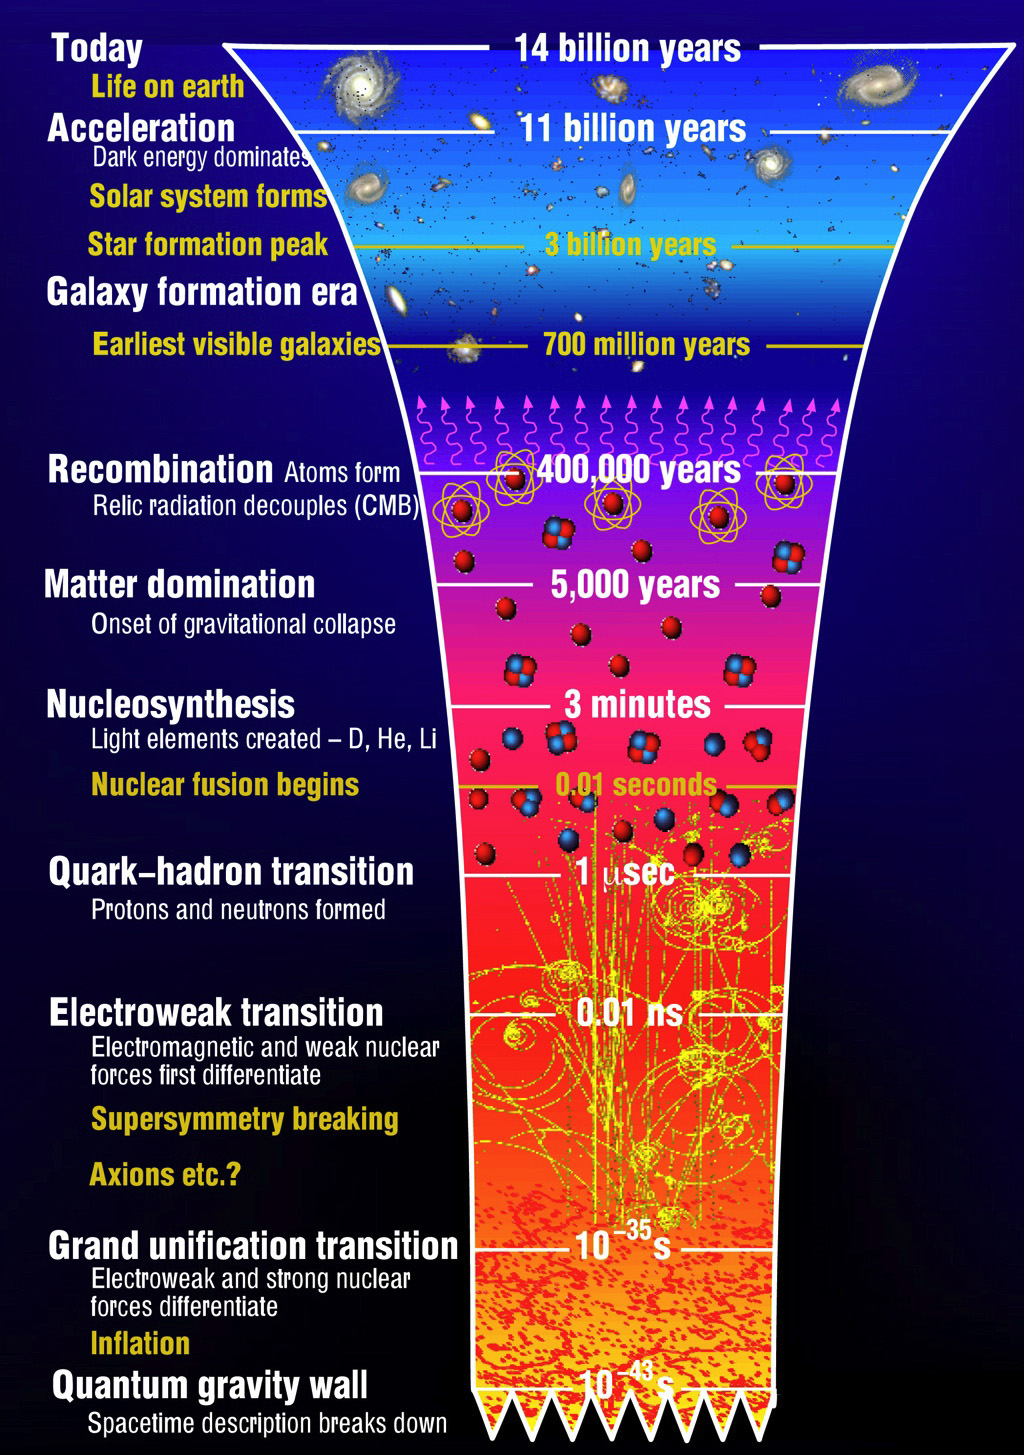
\includegraphics[width=8cm]{Chapter2/big_bang_timeline.png}
\caption{Big-Bang timeline.}
\label{fig:BigBang}
\end{center}
\end{figure}

The Large Hadron Collider~\cite{Bruning:782076, Evans:2008zzb} as the name suggests is a large circular accelerator having a circumference of $\sim$ 27\unit{km}
which accelerates counter rotating beams of hadrons and collides them to study the fundamental properties and interactions of quarks, leptons and bosons.  
It is the world's largest and most complex particle accelerator ever built. Earlier particle accelerators like ``Large Electron Positron'' collider
(LEP)~\cite{LEP} at CERN (in the same tunnel where LHC has been built) and Tevatron~\cite{Holmes:2011ey} at Fermilab, Batavia, IL, USA,
have been extensively used to confirm the predictions and test the precision of Standard Model parameters. Both of these were circular colliders.
The LEP was an $e^{+}e^{-}$ collider with a center of mass energy ($\sqrt{s}$) ranging from 90\unit{GeV} to 209\unit{GeV}
while Tevatron was a $\textrm{p}\bar{\textrm{p}}$ collider with $\sqrt{s}$ $=$ 1.8\unit{TeV} and 1.96\unit{TeV}.   
Studying a collision data obtained from electron-positron beam is far more easier as compared to proton beams due to the absence of hadronic background in the former.
However, in a circular ring of a particular radius, the loss of energy caused by synchrotron radiations is given as:
\begin{equation}
  -\Delta{E} = \frac{4{\pi}{\alpha}}{3r}\beta^{3}\gamma^{4} \:\:\: (\beta = v/c \simeq 1 \:\: \textrm{and} \:\: \gamma = E/mc^{2} \:\: \textrm{for relativistic speeds}),
  \label{eq:synchro}
\end{equation}
which is very large due to small mass of $e^{+}$ and $e^{-}$ and further increases as the speed $v$ approaches the speed of light $c$.
The choice is to either increase the radius of the circular rings or to use linear colliders or use heavy
particles in collision beams. The first two instances are not very easy to meet either due to technical or financial constraints,
so in order to achieve very high energies, proton beams are used. Since $m_{p}$ $\simeq$ $2000\:m_{e}$, use of proton beam reduces
synchrotron losses by a factor of ${(2000)}^{4}$ $\simeq$ $10^{13}$.

The requirement of very high energies for particle accelerators can be explained by the fact that in scattering experiments, the wavelength
of the probe should be smaller than the target particle size in order to observe the particle. Since, in particle physics, we look for extraordinarily small
entities, we need probes of smaller wavelengths or higher energies (as per the de broglie's relation, $\lambda$ = $\frac{h}{mv}$).
%However, measuring w.r.t macroscopic standards, these energies are not really large e.g. a center of mass energy of 14\unit{TeV} (designed center of mass
%energy of LHC) is equivalent to approximately one millionth of a joule which is just the energy consumed by a light bulb of 60\unit{W} power in
%around 20\unit{ns}. Actually, it is not the total energy but the energy per particle that matters here. In a light bulb, the
%total energy is distributed among a huge number of photons so each photon share a very little amount.
%But at LHC, each colliding proton has an energy of 7\unit{TeV} which definitely is very uncommon and huge.

\subsection{LHC tunnel layout}
The LHC is situated in an underground tunnel having a circumference of 26.7\unit{km} and a diameter of 3.8\unit{m}
at a depth of around 45 to 170\unit{m} beneath the France-Switzerland border. The LHC tunnel is divided in eight straight sections,
each of 528\unit{m} separated by eight arcs. The straight sections are utilized as experimental or utility insertions. 
A schematic diagram representing the layout of LHC tunnel is shown in \fig{\ref{fig:LHClayout}}. 
\begin{figure}[h]
\begin{center}
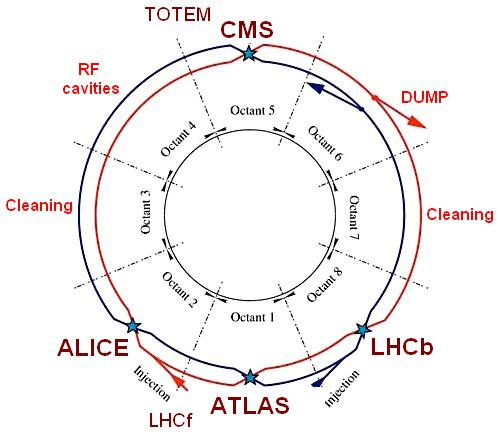
\includegraphics[width=9.6cm]{Chapter2/LHClayout.jpg}
\caption{A schematic layout of the LHC tunnel.}
\label{fig:LHClayout}
\end{center}
\end{figure}
%\vspace{-0.3in}

The eight sections are numbered from 1 to 8. The two general purpose detectors, namely,
A Toroidal LHC ApparatuS (ATLAS)~\cite{atlasTDR} and Compact Muon Solenoid (CMS)~\cite{cmsTDR} are located at point 1 and point 5 respectively. 
Point 2 is occupied by the heavy ion detector, A Large Ion Collider Experiment (ALICE)~\cite{aliceTDR} while the detector for b-physics
study, Large Hadron Collider beauty (LHCb)~\cite{lhcbTDR} is placed at point 8. These two points also have the beam injection utility for the two beams.
Collimation systems utilized for beam cleaning are placed at point 3 and 7 while the radio frequency (RF) systems for each beam are present at point 4.  
The point 6 has been used for the beam dump where the two beams are extracted vertically using horizontally and vertically deflecting magnets.
The LHC is primarily a proton-proton collider, but it also uses heavy ion beams to perform proton-lead and lead-lead collisions for some short periods of time.

\subsection{Main components of the LHC}
The design of LHC depends on very basic physics principles associated with latest technology. 
The three main components of LHC are:
\vspace{-0.1in}
\begin{enumerate}[leftmargin=*]
\item {\bf{Radio Frequency (RF) cavities}}: The RF cavities are located along the beam pipe and are used to provide acceleration to the 
  proton beams using alternating electric field. There are two independent RF systems, one for each beam. A sketch of a RF cavity is shown in the \fig{\ref{fig:RFcavity}}
  below.
  
  \begin{minipage}{0.55\textwidth}
  \begin{figure}[H]
    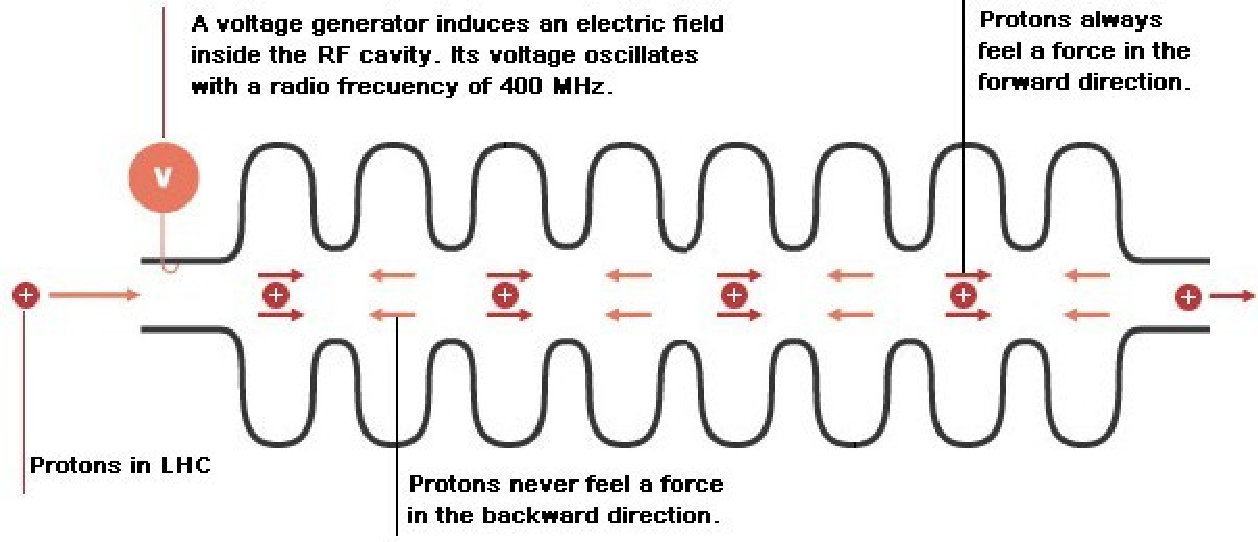
\includegraphics[width=9cm]{Chapter2/RFcavity.pdf}
    \caption{\label{fig:RFcavity} A Radio Frequency cavity.}
  \end{figure}
  \end{minipage}%
  \hfill
  \begin{minipage}{0.35\textwidth}
  \begin{figure}[H]
    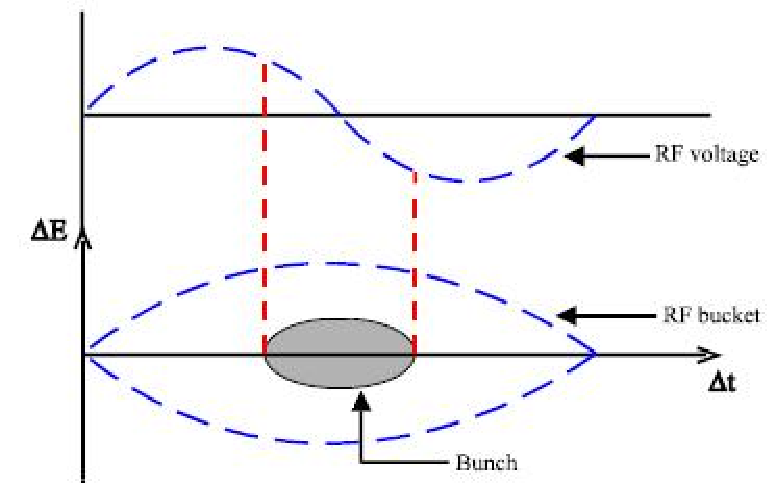
\includegraphics[width=6cm]{Chapter2/RFbucket.pdf}
    \caption{\label{fig:RFbucket} A sketch showing formation of a bunch.}
  \end{figure}
  \end{minipage}
  \vspace{0.1in}
  
  The sinusoidal varying alternating electric field of RF cavity changes polarity after each half cycle which implies that it accelerates the protons during one
  half cycle and decelerates during the other half. This results into the formation of bunches of protons. As can be seen in \fig{\ref{fig:RFbucket}}, when a proton
  arrives inside a RF cavity at a time when the voltage is zero, it will see no force and is called synchronous proton.
  Any proton arriving before the synchronous proton will see a negative polarity and hence will decelerate while any proton arriving later than
  the synchronous proton will see positive polarity and will get accelerated, so these protons will come closer to the synchronous proton and form a bunch.
  At LHC, the RF cavities resonate at a frequency of 400\unit{MHz}. The LHC is designed to have a total of 2808 bunches at a gap of 25\unit{ns}.
  The main goal of RF cavities is to maintain the tightness of proton bunches to provide high luminosity at collision points. These cavities also transfer
  the radio frequency power to the beam to provide acceleration. The LHC has eight RF cavities per beam operating at 4.5$^{^{\circ}}$\unit{K},
  each delivering a power of 2\unit{MV} at 400\unit{MHz}. 
    
\item {\bf{Vacuum chamber}}: The beam pipe in which proton beams travel are kept at a low pressure of $\sim$ $10^{-13}$ bar, much less
  than the outer space, forming an ultrahigh vacuum. This is required to minimize the interactions with parasitic particles and subsequent loss of
  accelerated protons. 
\item {\bf{Magnet system}}: In order to provide proper bending and focusing of the proton beams, an intense magnetic field varying in the range of 0.54\unit{T}
  (for 450\unit{GeV} proton energy) to 8.33\unit{T} (for 7\unit{TeV} proton energy) has been used. This high magnetic field has been achieved by the use of superconducting
  magnets made of copper plated Niobium-Titanium (NbTi) superconductors. The superconducting state has been attained by using many tones of superfluid Helium
  cooled to a temperature of 1.9$^{^{\circ}}$\unit{K}. Due to the constraints of small tunnel diameter, it was not possible to make completely
  separate rings for both the proton beams. So an alternate way was adopted in the form of twin-bore magnet design (a front view is shown in \fig{\ref{fig:LHCmagent}})
  which comprises of two coils and beam pipes
  at a separation of 180\unit{mm} within the same mechanical framework. This magnet structure is constructed in such a way that it provides
  opposite magnetic fields in the two beam pipes. The copper plated NbTi filaments are joined together to make the cables and two layers of these cables
  are wrapped around each beam pipe. The current is made to flow in opposite directions through the cables around the two pipes, which produces an intense magnetic field
  of opposite polarity in both the beam pipes. The copper provides an insulation among the NbTi filaments in superconducting state and act as a
  conductor upon reaching the conducting state.
  \begin{figure}[h]
  \begin{center}
  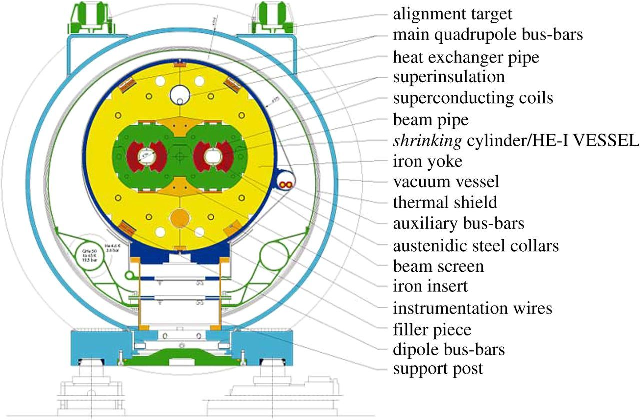
\includegraphics[width=12cm]{Chapter2/LHCmagnet.pdf}
  \caption{The LHC twin-bore magnet system}
  \label{fig:LHCmagent}
  \end{center}
  \end{figure}
%  \vspace{-0.3in}

  The LHC consists of different type of magnets that include, dipoles used for bending of the particle's beam,
  quadrupoles used for focusing of the beam, sextupoles and octupoles used for
  correcting the size and position of the beam. The LHC ring consists of 1232 dipoles, 392 quadrupoles and many sextupoles and octupoles.
  To enhance the probability of collisions, the bunches are squeezed by the use of special magnets positioned
  near the collision chambers. These magnets reduce the beam diameter to a minimum of 16 $\mu$m.

\end{enumerate}

\subsection{Proton's journey to maximum acceleration}
Making the proton beams travel closer to the speed of light is a very intricate task. At LHC, it has been accomplished
in a number of steps as can be seen in the schematic representation of CERN accelerator complex~\cite{Web:CERN} in \fig{\ref{fig:LHCring}}.
%\vspace{-0.15in}
\begin{figure}[h]
\begin{center}
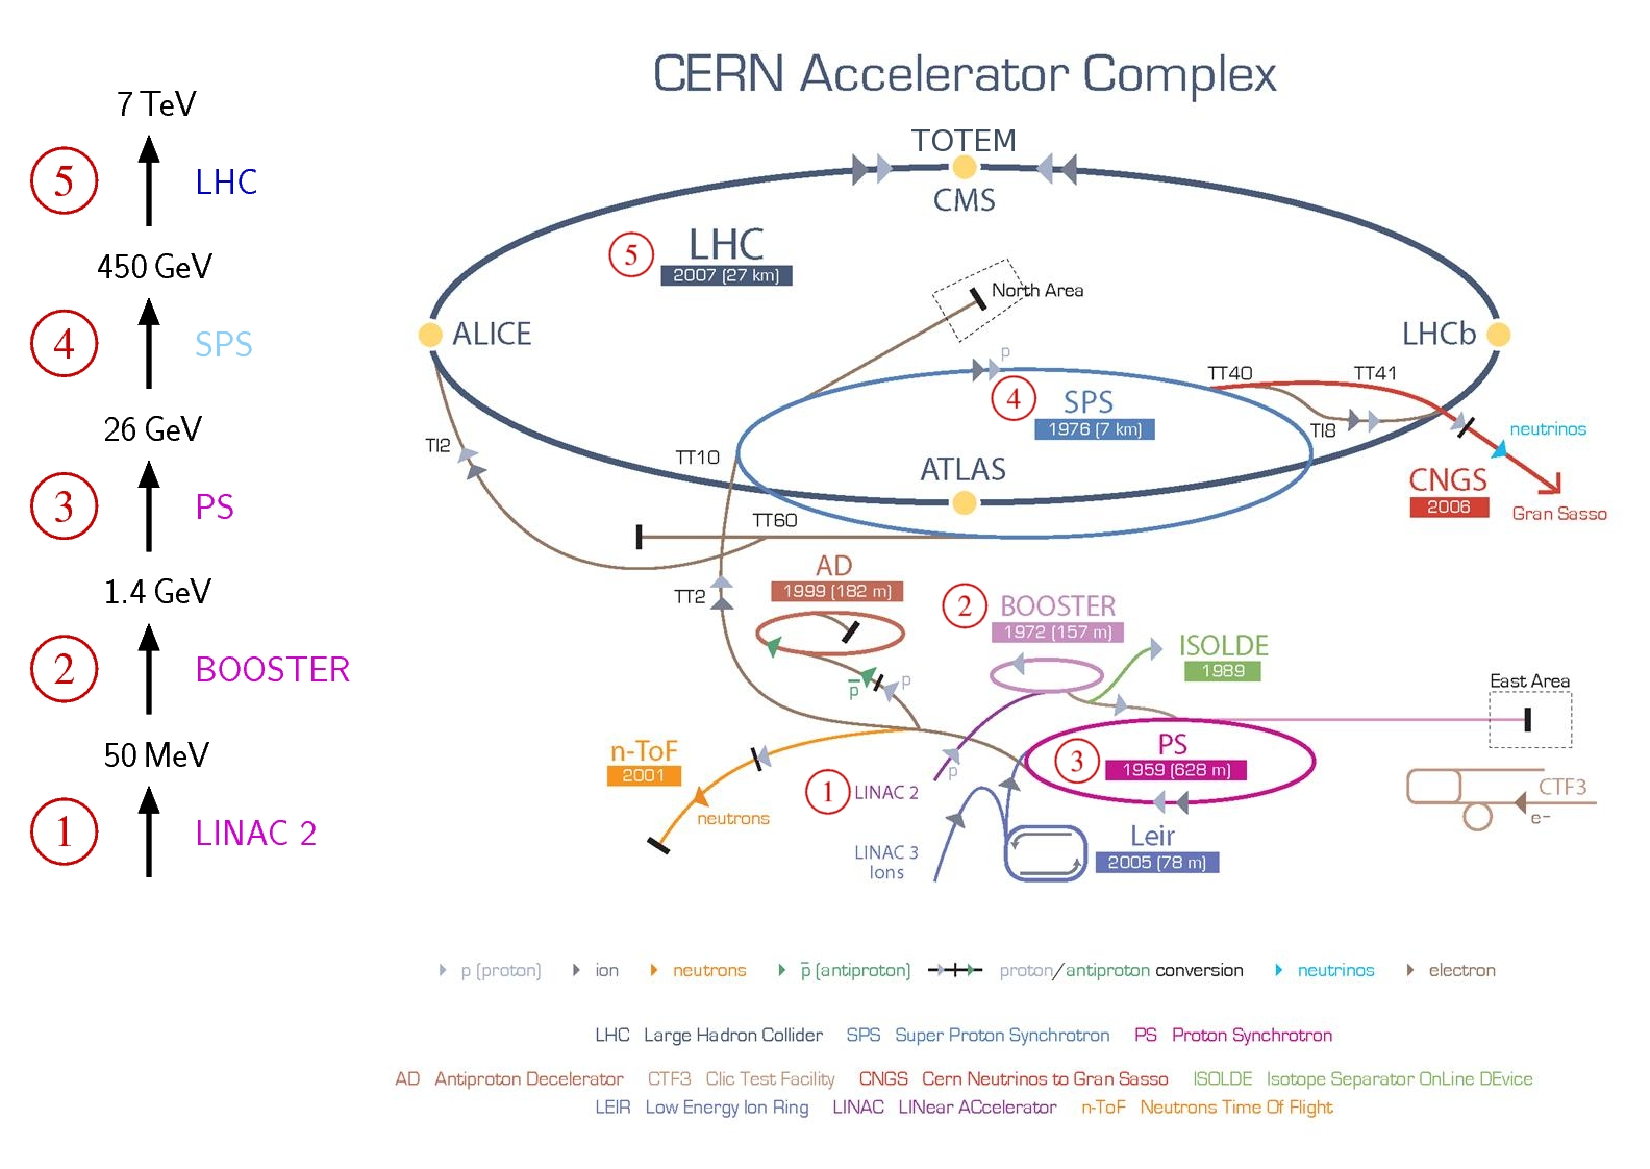
\includegraphics[width=14cm]{Chapter2/LHCRing3.pdf}
\caption{A schematic view of CERN accelerator complex representing the different accelerators deployed for providing acceleration to the proton beam.}
\label{fig:LHCring}
\end{center}
\end{figure}
%\vspace{-0.3in}
First of all, protons are extracted from hydrogen gas by stripping off the electrons using an electric discharge. Then, the protons
are directed towards a Radio Frequency Quadrupole (QRF) that provides an initial acceleration of 750\unit{keV} to the beam. After that, the protons are sent to
LINAC2, a linear accelerator that makes use of RF cavities and accelerates the proton beam upto 50\unit{MeV}. The beam from LINAC2 is made to enter
Proton Synchrotron Booster (PSB) which increases the energy of protons to 1.4\unit{GeV} and divides the proton beam into 6 bunches.
The output of PSB is then injected into Proton Synchrotron (PS) that accelerates the protons upto 25\unit{GeV}.
The PS is also responsible for preparing the LHC bunch structure. A total of 72 bunches with a spacing of 25\unit{ns} are formed in PS. The proton bunches from PS
then enter into Super Proton Synchrotron (SPS) where they are further bunched into 288 bunches and are accelerated upto the LHC injection energy of 450\unit{GeV}.
The protons from SPS are then finally made to enter into LHC where they accelerated upto the highest energy required.

\subsection{Luminosity measurements at LHC}
At LHC, the rate of collision N is expressed in terms of the instantaneous luminosity $L$ as $N$ = ${\sigma}L$ where $\sigma$ is the cross section of
the process under study. For a given process, the higher the luminosity, the
chances are more of a collision to happen. The luminosity of a beam depends upon many machine parameters and is given by,
\begin{equation}
  L = \frac{N^{2}_{b}n_{b}f_{rev}\gamma_{r}}{4\pi\beta^{\ast}\epsilon_{n}}F, 
\end{equation}
where, \\
$N_{b}$: number of particles in a bunch,\\
$n_{b}$: number of bunches in each beam,\\
$f_{rev}$: beam revolution frequency,\\
$\gamma_{r}$: relativistic gamma factor,\\
$\epsilon_{n}$: normalized transverse beam emittance\footnote{The beam emittance is defined as the transverse size of the beam. The narrower the beam, the lesser
  is the beam emittance and more are the chances of interaction.},\\
$\beta^{\ast}$: betatron function\footnote{Betatron function is defined as the distance from the
  collision point at which the beam width in transverse plane is twice compared to the beam width at collision point.}, and\\
$F$: luminosity reduction factor due to the presence of crossing angle between the two beams.
%\begin{equation}
%F = \left(1+\left(\frac{\theta_{c}\sigma_{z}}{2\sigma^{\ast}}\right)\right)
%\end{equation}

In order to achieve highly luminous beams, one need to provide large number of highly populated bunches
having low value of beam emittance and betatron function colliding at high frequencies. The various parameters related to LHC machine and proton beams
are summarized in \tab{\ref{Table:LHCParameters}}.
\begin{table}[h!]
\begin{center}
\resizebox{13cm}{!}{
%\begin{tabular}{c !{\vrule width -1pt}c !{\vrule width -1pt}c !{\vrule width -1pt}c !{\vrule width -1pt}c !{\vrule width -1pt}c !{\vrule width -1pt}c !{\vrule width -1pt}c}  %%% !{\vrule width -1pt} to make column line width less, so that white space not visible in colored table. but not working very nicely.
\renewcommand{\arraystretch}{1.2}
\begin{tabular}{lcc}
\toprule
\belowrulesepcolor{Mygray}
\belowrulesepcolor{Mygray}
\belowrulesepcolor{Mygray}
\rowcolor{Mygray}[\dimexpr\tabcolsep+0.09pt\relax]  
LHC Parameters  & Design Value & 2016 Value \\
\aboverulesepcolor{Mygray}
\aboverulesepcolor{Mygray}
\aboverulesepcolor{Mygray}
\midrule
Total number of magnets & 9600 & -- \\
Number of dipole magnets & 1232 & -- \\
Beam energy (TeV) & 14 & 13 \\
Bunch spacing (ns) & 25 & 25 \\
No. of protons per bunch & 1.1 $\times$ $10^{11}$ & 1.1 $\times$ $10^{11}$ \\
No. of bunches per beam & 2808 & 2220 \\
Beam crossing angle ($\mu$rad) & 285 & 370 \\
Beam emittance, $\epsilon_{n}$ ($\mu$m) & 3.75 & 3.4 \\
Betatron function, $\beta^{\ast}$ (m) & 0.55 & 0.4 \\
Instantaneous luminosity (cm$^{-2}$sec$^{-1}$) & 1.0 $\times$ $10^{34}$ & 1.0 $\times$ $10^{34}$ \\
\bottomrule
\end{tabular}
}
\caption{Design values of the various parameters of LHC and a comparison with the values obtained during the 2016 run.}
\label{Table:LHCParameters}
\end{center}
\end{table}
\vspace{-0.4in}


The sum of instantaneous luminosities obtained over a period of time is referred to as the integrated luminosity. The \fig{\ref{fig:LHCLumi}} shows
the total integrated luminosity delivered by the LHC and recorded by CMS~\cite{Web:CMSLumi} over a period of time for the year 2016.

\begin{figure}[h]
\begin{center}
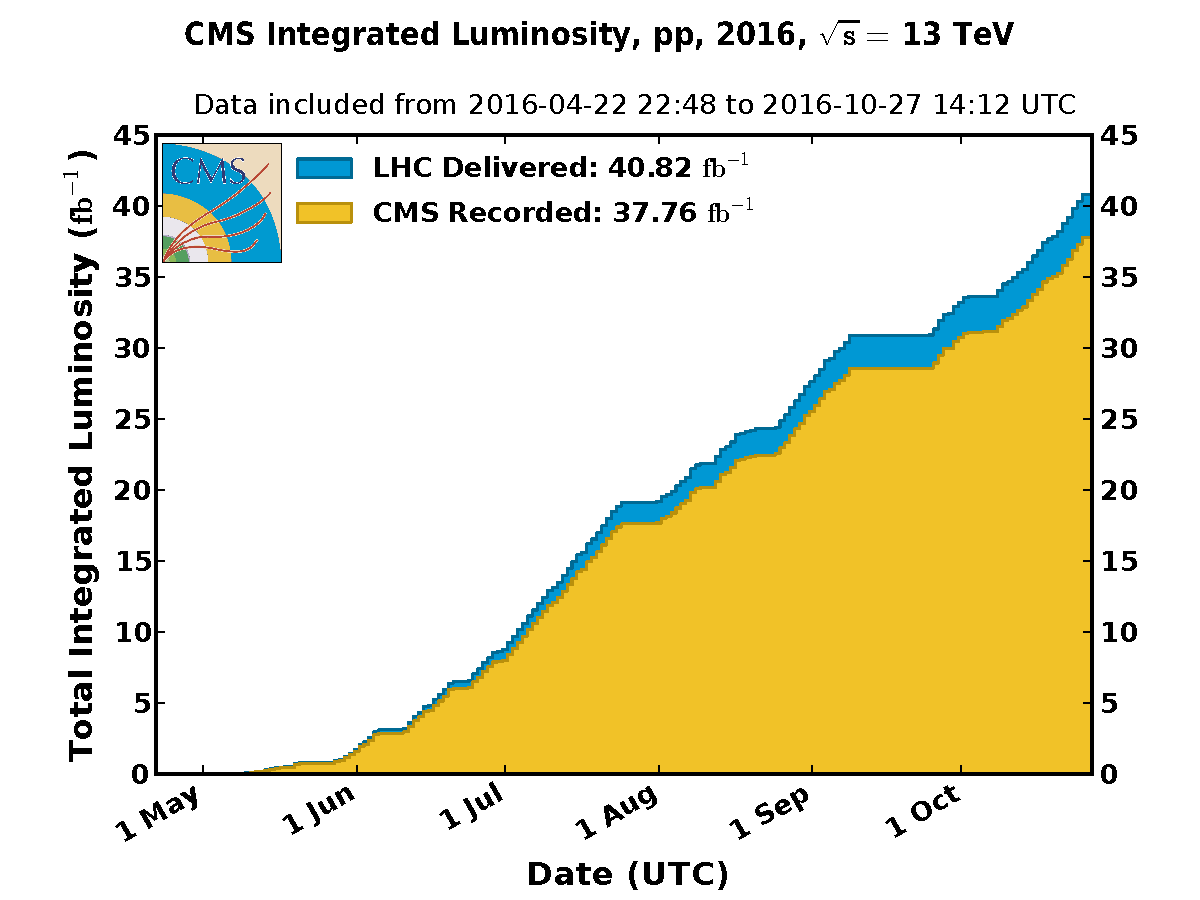
\includegraphics[width=8.6cm]{Chapter2/Int_lumi_offline_pp_2016.pdf}
\caption{Total integrated luminosity delivered by the LHC and recorded by CMS as a function of time, during the year 2016~\cite{Web:CMSLumi}.}
\label{fig:LHCLumi}
\end{center}
\end{figure}
%\vspace{-0.3in}

During the 13\unit{TeV} run in 2016, the LHC delivered a total of 40.8\fbinv of pp collision data, out of which, CMS recorded a total of 37.8\fbinv.
The CMS has certified 35.9\fbinv of recorded data to be used for physics analysis. The study presented in this thesis has been performed using this 35.9\fbinv
of data.

%%%%%%%%%%%%%%%%%%%%%%%%%%%%%%%%%%%%%%%%%%%%%%%%%%%%%%%%%%%%%%%%%%%%%%%%%%%%%%%%%%%%%%%%%%%%%%%%%%%%%%%%%%%%%%%%%%%%%%%%%%%%%%%%%%%%%%%%%%%%%%%%%%%%%%%%%%%%%%%%%%%%%%%%%%%%
%% The LHC has first started functioning in September, 2008 but halted 9 days later because of a magnet quench and helium gas explosion. It started
%% again in November, 2009 and began its first ever data taking. It recorded good physics runs for a period of around three years from March, 2010
%% to February, 2013 at a center of mass energy of 7 and 8\unit{TeV} (known as Run 1). Around $20$\fbinv\ of data collected at 8\unit{TeV} during this period
%% showed the first evidence of much awaited Higgs boson. After the Run 1, the accelerator was shut down (known as Long Shutdown 1, LS1) for next two
%% years for upgradation. It restarted again during second half of 2015 and began data taking at an increased center of mass energy of 13\unit{TeV}.
%% Its next long shut down (LS2) is scheduled to happen from 2019, it is aiming to record a data of around $100$\fbinv before that.                              
%%%%%%%%%%%%%%%%%%%%%%%%%%%%%%%%%%%%%%%%%%%%%%%%%%%%%%%%%%%%%%%%%%%%%%%%%%%%%%%%%%%%%%%%%%%%%%%%%%%%%%%%%%%%%%%%%%%%%%%%%%%%%%%%%%%%%%%%%%%%%%%%%%%%%%%%%%%%%%%%%%%%%%%%%%%%


\section{The CMS Detector}
The CMS detector~\cite{Chatrchyan:2008aa} is one of the main particle detectors designed at the LHC to observe different kind of particles and processes
produced in the pp collisions. The prime objective of the CMS detector is to explore the physics at Terascale, the energy region at which the physicists believe
the experiment has the potential to answer some of the existing key questions. The detector has a cylindrical onion like structure having a coverage of $4\pi$ steradian,
with each layer representing a different sub-detector used to measure different type of particles. The information from different layers is used to build up
the complete picture of an event. It is situated in a cavern, 100\unit{m} underground, located at point 5 of the LHC tunnel in France near village Cessy.
It has a length of 21.6\unit{m} and a diameter of 14.6\unit{m}, it weights around 14,000 tonnes.
CMS is a large scientific collaboration involving around 3,000 people from 198 scientific institutions and universities belonging to 45 countries.

\noindent
{\bf{Experimental challenges}}:\ As discussed in last section, the LHC has a very high collision rate which is achieved by colliding bunches of more than 100 billion
protons each, 40 million times every second, resulting into a pp interaction rate of around $10^{9}$ per second.
The high track density arising due to these interactions create severe radiation environment. The detector needs to remain unaffected from these radiations along with
providing efficient particle identification. The detector has to face the challenge of adjusting between occupancy and granularity.
Additionally, a majority of collisions contain uninteresting events, a fast filtering trigger system is required to reject these unwanted events.
Also, the interesting pp events are superimposed by many uninteresting events occurring in the same bunch crossing (known as pile-up).
Dealing with these events require high granularity and good time resolution detectors, which further demand to have large number of detector channels with
good synchronization. Even storing the data after huge reduction require about 10 million gigabytes per year which in itself is a big challenge.

\subsection{Layout of the CMS detector}
A general layout of the CMS detector is presented in \fig{\ref{fig:CMS_layout}}. It is based on four principle sub-systems: A high granularity central tracker,
a homogeneous electromagnetic calorimeter, a sampling hadron calorimeter and a muon detector. The heart of the CMS is its very high superconducting magnet
that is situated between the calorimeters and the muon detector. All the sub-systems of the detector are divided into one cylindrical barrel region and
two opposite facing endcap regions, complimented with very forward regions.
This arrangement provides a very good coverage of the collision fragments required for event building. A longitudinal view of the CMS detector system,
showing the barrel and endcap sections of various sub-detectors is presented in \fig{\ref{fig:CMS_longitudinal}}, with the origin denoting the interaction point.
\vspace{0.2in}

\begin{figure}[t]
\begin{center}
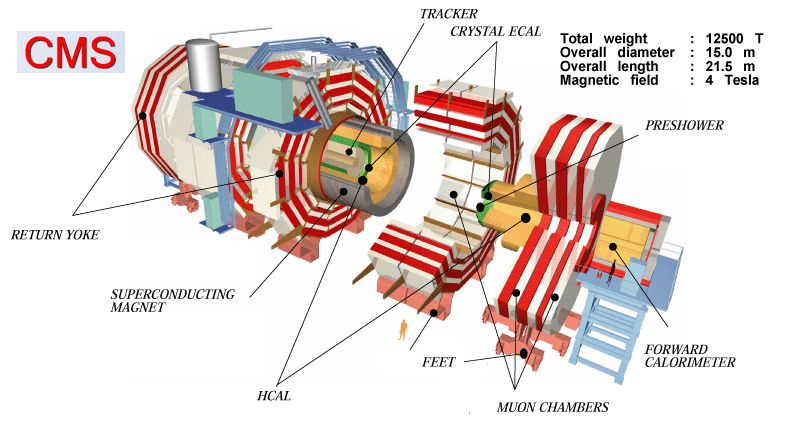
\includegraphics[width=15cm]{Chapter2/CMS_layout.png}
\caption{A layout of the CMS experiment at CERN.}
\label{fig:CMS_layout}
\end{center}
\end{figure}
%\vspace{-0.3in}


\begin{figure}[h]
\begin{center}
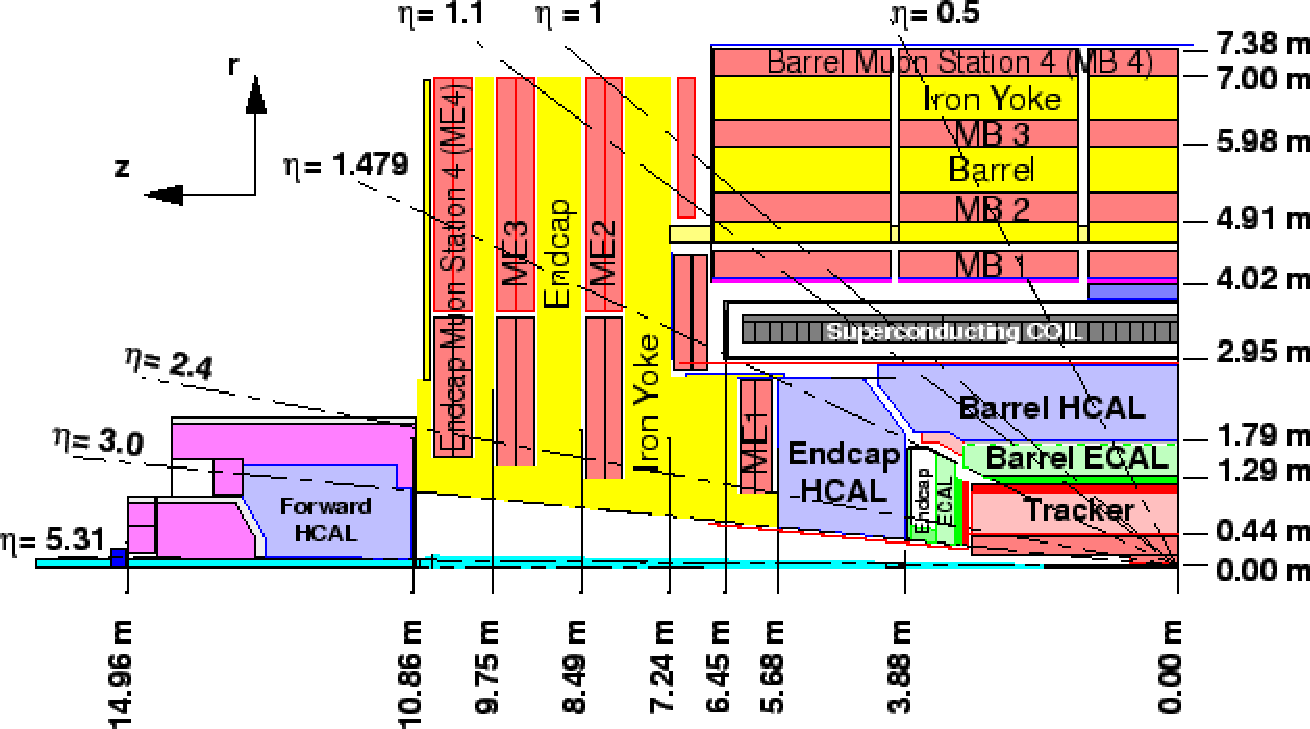
\includegraphics[width=12cm]{Chapter2/CMS_longitudinal.pdf}
\caption{Longitudinal contour of a quadrant of the CMS detector.}
\label{fig:CMS_longitudinal}
\end{center}
\end{figure}
\vspace{-0.2in}

\noindent
{\bf{Co-ordinate system}}: The CMS has adopted a right-handed spherical co-ordinate system with origin at the center of the detector which is also the
intended collision point. The $x$-axis points towards the center of the LHC tunnel, the $y$-axis is vertically upwards and the $z$-axis is along the beam pipe.
The polar angle $\theta$ is taken from the $z$-axis to the $x$-$y$ plane and the azimuthal angle $\phi$ is taken from the $x$-axis to the $y$-axis in the $x$-$y$ plane.
The angle $\theta$ denotes the particle's angle w.r.t the beam axis while angle $\phi$ denotes the particle's orientation in the transverse plane.
The co-ordinate $r$ denotes the radial distance and is defined by $r$ = $\sqrt{x^{2}+y^{2}+z^{2}}$.
It is conventional to use pseudorapidity $\eta$ instead of polar angle $\theta$ as 
seen in \fig{\ref{fig:CMS_longitudinal}}. The pseudorapidity is defined in terms of angle $\theta$ as
\begin{equation}
  \eta = -\ln\left[\tan\frac{\theta}{2}\right].
\end{equation}
On going from -$z$ to +$z$ axis, $\theta$ goes from -$\pi$ to +$\pi$ and $\eta$ goes from -$\infty$ to +$\infty$. In the non-relativistic limit,
it is called rapidity and is defined as,
\begin{equation}
  y = \frac{1}{2}\ln\left(\frac{E + p_{z}}{E - p_{z}}\right),
\end{equation}
where $E$ and $p_{z}$ are the particle's energy and $z$-component of the momentum. The rapidity, $y$ requires the measurement
of both $E$ and $p_{z}$ and in relativistic regime, it is quite difficult to measure the $z$-component of momentum very precisely.
The reason of choosing $\eta$ over $\theta$ is that the difference between
the pseudorapidity of two particles ($\Delta\eta$) is Lorentz invariant under boosts along the beam axis. This means that an observer in the lab frame, boosted
along $z$-axis w.r.t the rest frame, will measure the same $\Delta\eta$ between two particles as an observer in the rest frame.
The importance of this feature comes from the fact that in the pp collisions, the hard interaction takes place between proton constituents (quarks or gluons),
usually having different momenta, which means the different interactions have different boosts of their center-of-mass frames w.r.t the detector rest frame.
Invariance of $\Delta\eta$ under boosts allows us to treat the different interactions in a similar way as the interaction happening in the center-of-mass rest frame.
The various histograms binned on the angular separation of particles will remain undistorted by these arbitrary boosts of different events.
The angular distance $R$ between two particles in $\eta-\phi$ plane, as observed from the origin of CMS detector,
is written in terms of the differences in $\eta$ and $\phi$ as, $R$ = $\sqrt{({\Delta\eta})^{2}+({\Delta\phi})^{2}}$.

In colliders, two particle beams colliding head-on consist of only longitudinal component of momentum. So the particles in the beam do not have a transverse component
of momentum before collision, thus by conservation of momentum, the total transverse momentum after the collision should also add up to zero. This feature is
extensively used in collider experiments and it requires to consider the
particle's energy and momentum in the transverse direction, known as transverse energy (\et) and transverse momentum (\pt), defined as
\et = $E\sin\theta$ and \pt = $\sqrt{p_{x}^{2} + p_{y}^{2}}$ respectively.  
Any imbalance in the transverse momentum is caused by either the invisible particles like neutrinos or by the energy lost in the unavoidable nuclear processes.
This imbalance is known as missing transverse energy and is given by, \met = -$\sum{\pt}$.
    
A short description of all the components of the CMS detector from innermost to outermost has been provided as follows:

\subsubsection{CMS tracking system}\label{Se:CMS_tracker}
The tracker~\cite{Chatrchyan:2008aa,Karimaki:368412} is the innermost sub-detector, installed close to the interaction point. It has been designed to
build tracks of charged particles coming out of the collisions and reconstruct primary as well as secondary vertices, with utmost precision and accuracy.     

The tracker has a total length of 5.8\unit{m}, a diameter of 2.5\unit{m} and covers a region upto $|\eta|$ $<$ 2.5.
A uniform magnetic field of 3.8\unit{T} is present over its entire volume. 
A cross-sectional view of the CMS tracker has been presented in \fig{\ref{fig:CMS_tracker}}. The tracker is made up of a central barrel and
endcap parts consisting of pixel and strip layers. Both pixel and strip layers are made up of silicon sensors of different dimensions.
The CMS tracker is the world's largest silicon tracker with over 200$\unit{m}^{2}$ of active silicon area. 
Whenever a charged particle passes through a silicon sensor, it results into generation of electron-hole pairs,
which are measured in an outer circuit as a hit. Subsequent information of the large number of hits from different sensors
leads to the reconstruction of the particle's track.
Since the energy required to generate an electron-hole pair is small, the energy$/$momentum resolution of these sensors
is very large. Also, since the electrons travel very fast to the outer circuit, the time resolution is better. 
The charged particles of different momentum curved differently under the effect of
the magnetic field and the tracker records the particle's tracks and momentum by finding their positions and curvature at various key points.  

\begin{figure}[h]
\begin{center}
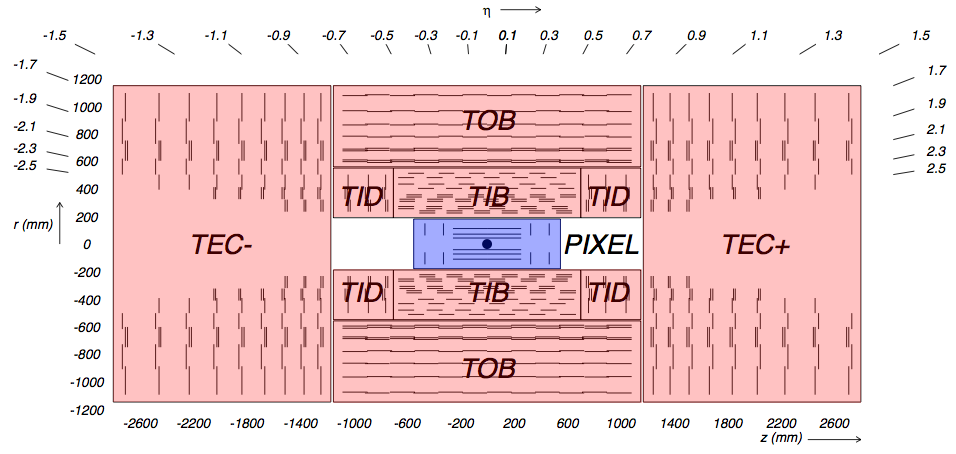
\includegraphics[width=13.4cm]{Chapter2/CMS_tracker.png}
\caption{A cross-sectional view of the CMS tracker system in $r$-$z$ plane, with each line representing a silicon detector module.}
\label{fig:CMS_tracker}
\end{center}
\end{figure}
\vspace{-0.3in}

The tracker has to face around 1000 particles coming from each bunch crossing at every 25\unit{ns} which lead to high radiation doses in the detector. So it should
be able to operate in such a harsh environment in addition to dealing with high occupancy rate as well as providing high granularity and
quick response~\cite{Chatrchyan:2014fea}. The silicon detector technology meets all these goals very efficiently. 
The number of tracker layers is a tradeoff among the tracking efficiency and material budget~\cite{CMS:2010nua}.
On one side, more layers leads to more hits and precise track reconstruction. While on other side, large amount of
material inside the tracker leads to multiple scattering which in turn can spoil proper tracking too.

In order to reconstruct a track using hits, the simplest approach is to start from a hit in the innermost layer and in radial direction, project a cone on the next layer.
If the next layer contains no hit within the cone, leave the starting point considering it a noise or a particle of very low energy. Otherwise, keep on repeating the
procedure until last layer is reached. A more advanced approach start the search from the outermost layer along with taking additional information from other sub-detectors.
A description of pixel and strip layers of CMS tracker has been provided below.

\paragraph {\bf{Pixel detector}}
\hspace{\parindent} The high precision pixel detector~\cite{Baur:1999tw} is the innermost detector of the CMS tracker. Since the particle flux near
the collision point is very large, a small-scale pixel geometry is constructed to achieve unambiguous track reconstruction and precise vertex determination.
The particles with relatively long lifetime, such as b and c quarks, arise from primary vertex but decay after travelling small distances, forming secondary
vertices. The pixel detector is designed to distinguish these secondary vertices from the primary collision point.

The pixel detector consists of three concentric barrel layers and two endcap disks on both sides (shown in \fig{\ref{fig:CMS_PixelDet}}),
covering a pseudorapidity region of $|\eta|$ $<$ 2.5. The barrel layers are 
53\unit{cm} long and are present at the radii of 4.4, 7.3 and 10.2\unit{cm} from the beam line. The two endcap disks are extended in radius from 6\unit{cm} to 15\unit{cm}
and are present at $\pm$34.5 and $\pm$46.5\unit{cm} from the collision point. The detector is equipped with a total of about 66 million pixels, each
having a size of 100$\times$150${\mu{m}}^{2}$.
The occupancy rate of each pixel is of the order of 0.1$\%$ per LHC bunch crossing.  

\begin{figure}[h]
\begin{center}
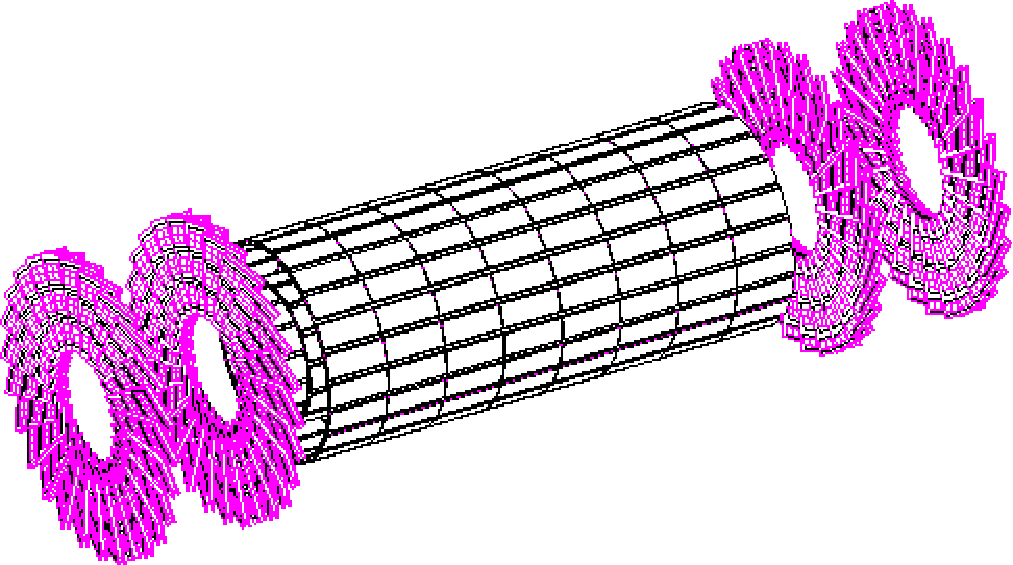
\includegraphics[width=8cm]{Chapter2/CMS_PixelDet.pdf}
\caption{A schematic layout of the CMS pixel detector.}
\label{fig:CMS_PixelDet}
\end{center}
\end{figure}

The pixel detector has performed exceedingly well during Run I, providing a resolution of
around 10{$\mu${m}} in $r-\phi$ and 20-40{$\mu${m}} in $z$
direction along with an overall efficiency of more than 99$\%$. The LHC Run II started in 2015 with an increased center of mass energy of 13\unit{TeV}
and a lower bunch crossing frequency of 25\unit{ns}. During overall Run II phase,
a peak instantaneous luminosity of 2 $\times$ $10^{-34}\unit{{cm}^{-2}{s}^{-1}}$ was achieved.
It also saw a pileup rate of more than 50. Under these conditions, the current pixel detector will suffer from increased fake rates and reduced resolution
due to higher occupancy. So in order to maintain the performance of pixel detector, an upgrade known as
``Phase1 Pixel Upgrade''~\cite{CMS:2012sda,1748-0221-9-03-C03041} was
performed during the technical stop at the end of 2016. The upgraded pixel detector features 4 barrel layers and a turbine-like module arrangement for endcap
disks (as shown in \fig{\ref{fig:Pixel_upgrade}}). Light-weight support structures and 2-phase CO$_{2}$ cooling has been introduced to keep the optimum material budget.  
A comparison of the two detector configurations using tracking efficiency and fake rate as a function of pileup are presented in \fig{\ref{fig:Pixel_upgrade_effects}}.

\begin{figure}[h]
\begin{center}
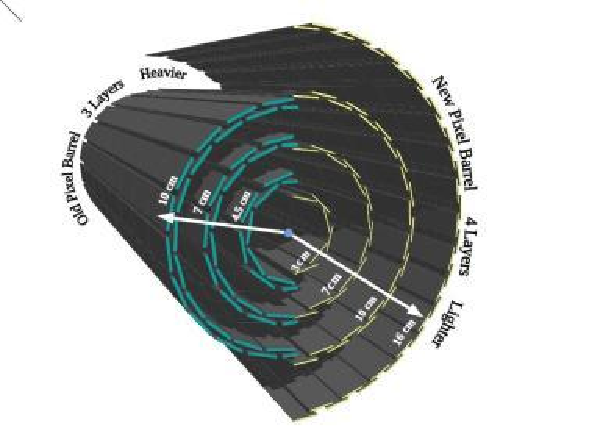
\includegraphics[width=7cm]{Chapter2/PixelDetector_barrel_oldvsNew.pdf}
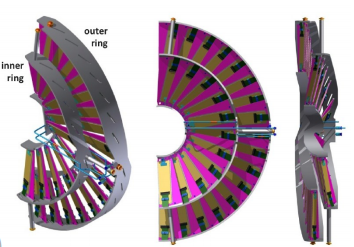
\includegraphics[width=7.5cm]{Chapter2/Pixel_upgrade_endcaps.png}
\caption{A schematic representation of the upgrades in pixel detector barrel (left) and endcaps (right) during Phase1 Pixel Upgrade.}
\label{fig:Pixel_upgrade}
\end{center}
\end{figure}
\vspace{-0.3in}

\begin{figure}[h]
\begin{center}
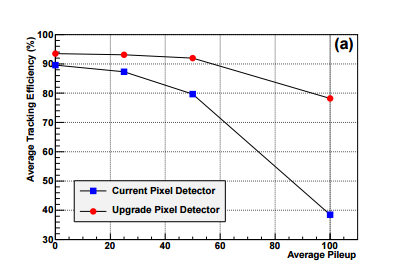
\includegraphics[width=7.2cm]{Chapter2/PixelUpgrade_trackEff.png}
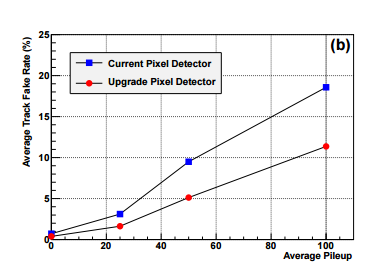
\includegraphics[width=7.2cm]{Chapter2/PixelUpgrade_fakerate.png}
\caption{Performance measurement of the older pixel detector (blue) and the upgrade pixel detector (red) using $\textrm{t}\bar{\textrm{t}}$ events,
  showing tracking efficiency (left) and fake rate (right) as a function of per event pileup~\cite{1748-0221-9-03-C03041}.}
\label{fig:Pixel_upgrade_effects}
\end{center}
\end{figure}

\paragraph {\bf{Silicon strip detector}}
\hspace{\parindent} The silicon strip tracker~\cite{Chatrchyan:2008aa,Karimaki:368412} is present outside the pixel detector
  and consists of more than 15000 single or double sided (shown in \fig{\ref{fig:CMS_tracker}} by single and double lines)
  modules. Since the particle flux reduces in strip tracker,
  the dimensions of strip modules are kept larger than that of pixel detector modules. The size of modules also increases with distance to keep the occupancy level
  at around 1$\%$. The modules are of rectangular shape in barrel region while that of trapezoidal shape in the endcap region.
  The strip tracker consists of four subsystems: The Tracker Inner Barrels (TIB), Tracker Inner Disks (TID), Tracker Outer Barrels (TOB) and
  Tracker EndCaps (TEC).

  The TIB and TID are extended up to a radius of 55\unit{cm} and consists of 4 barrel $+$ 3 endcap layers. The modules in TIB$/$TID are 320{$\mu${m}} thick and
  delivers up to 4 measurements in $r-\phi$ direction, providing a position resolution of 23{$\mu${m}} in the inner two layers and 35{$\mu${m}} in the outer two layers.
  The outer barrel layer TOB is made up of 6 layers of 500{$\mu${m}} thick sensors extended up to an outer radius of 116\unit{cm} which provides 6 more measurements
  in $r-\phi$ direction, corresponding to a resolution of 53{$\mu${m}} in the initial four layers and 35{$\mu${m}} in the last two layers.
  The TOB covers a $z$ range up to $\pm$118\unit{cm}.
  Outside this range, $\pm$TEC occupies the region from $124-282$\unit{cm} in ${\pm}z$ and $22.5-113.5$\unit{cm} in ${\pm}r$. Each of the TEC is made up of 9 disks, thereby
  providing 9 measurements in $r-\phi$ per trajectory. 

  The transverse momentum resolution of the tracker varies in the range from 0.7$\%$ at 1\unit{GeV} to 1.5$\%$ at 100\unit{GeV}.

\subsubsection{Calorimeter}
A calorimeter is a device that is used to measure energies of different type of particles. The incident particle interacts with the material of the calorimeter and
produces a cascade (shower) of secondary particles of progressively lower energies, until the energies fall below a critical value which is then
dissipated in ionization or excitation of the atoms of the material. The subsequent energy released by the atoms is captured by the photo-detector which through
photoelectric effect, yield an electronic signal that provides a measurement of the particle's energy.
In case of the sampling calorimeters, the medium that activate the particle shower is known as the passive medium (absorber)
while the one that absorb the shower particles and lead to the energy measurement, is known as the active medium (scintillator).
Calorimeters has the capability to stop almost all particles except muons and neutrinos. 

Calorimeters are broadly divided into two categories: Hadronic and Electromagnetic, depending on the particle type. They can also be classified
on the basis of their composition into sampling and homogeneous calorimeters. A sampling calorimeter is the one that consists of alternate layers of
two materials acting as passive and active mediums while a homogeneous calorimeter is build up of only one type of material that accomplish both the tasks.
An advantage of sampling configuration is that both the materials used are well-suited for their tasks. A very high density material is used as passive medium
which results into the quick evolution of the shower into a limited space, so sampling calorimeters can be made compact as compared to homogeneous calorimeters.
However, it has a disadvantage that part of the shower energy get deposited in the passive medium and left unmeasured. 

The CMS consists of Electromagnetic calorimeter (ECAL) just outside the tracker, followed by Hadronic calorimeter (HCAL), both contained inside the solenoidal magnet.
A short description of each one is considered below.

\paragraph{Electromagnetic calorimeter}
\hspace{\parindent}
The CMS ECAL measures the energy of electromagnetically interacting particles, primarily photons and electrons. The photons interact with the material of the detector
mainly through pair production for energies above 1\unit{MeV} and through Compton scattering and photoelectric effect for energies below 1\unit{MeV}.
On the other hand, electrons mainly interact via bremsstrahlung for energies above 10\unit{MeV} and through ionization and excitation for energies below it.
As a consequence, high energy electrons and photons, inside ECAL, produce a number of secondary particles, thereby generating electromagnetic (EM) showers.
The EM showers are characterized by a material dependent parameter, the radiation length denoted as $X_{0}$, which is the average distance $x$ travelled by an electron
before losing an energy equivalent to $1/e$ times its original energy \ie $E = E_{0}e^{-\frac{x}{X_{0}}}$.
It is also equivalent to $7/9$ times the free path travelled by photon before converting into an $e^{+}e^{-}$ pair.

As a result of particle multiplication and faster interaction, the amount of material required to contain an EM shower is rather small. Therefore,
the ECAL~\cite{Chatrchyan:2008aa, ecalTDR} (shown in \fig{\ref{fig:ECAL}})
is constructed as a homogeneous calorimeter made up of lead tungstate (PbWO$_{4}$) scintillating crystals.
It is a highly dense material (8.28$\unit{g/{cm}^{3}}$) with a radiation length of 0.89\unit{cm} and Moli$\grave{\textrm{e}}$re radius of 2.2\unit{cm},
allowing a design of fast, granular and radiation resistant calorimeter.
The crystals are designed to provide very good energy resolution of electrons and photons required for CMS physics program. 
These are arranged in carbon fibre matrices to provide optical isolation.  


\begin{figure}[h]
\begin{center}
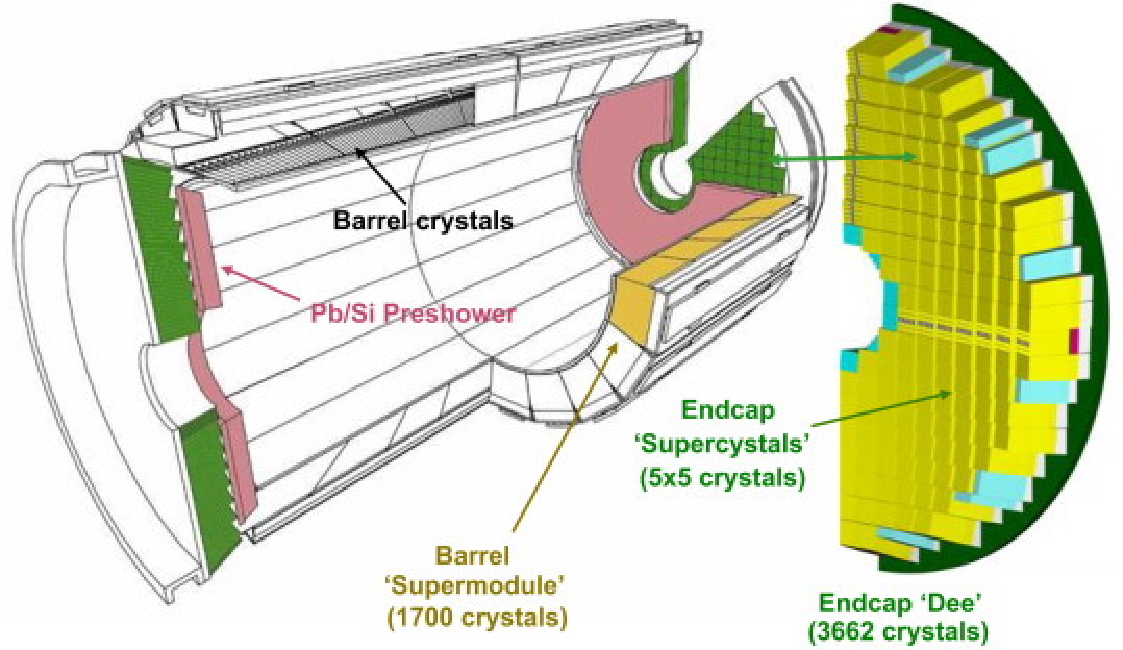
\includegraphics[width=11cm]{Chapter2/ECAL_layout.pdf}
%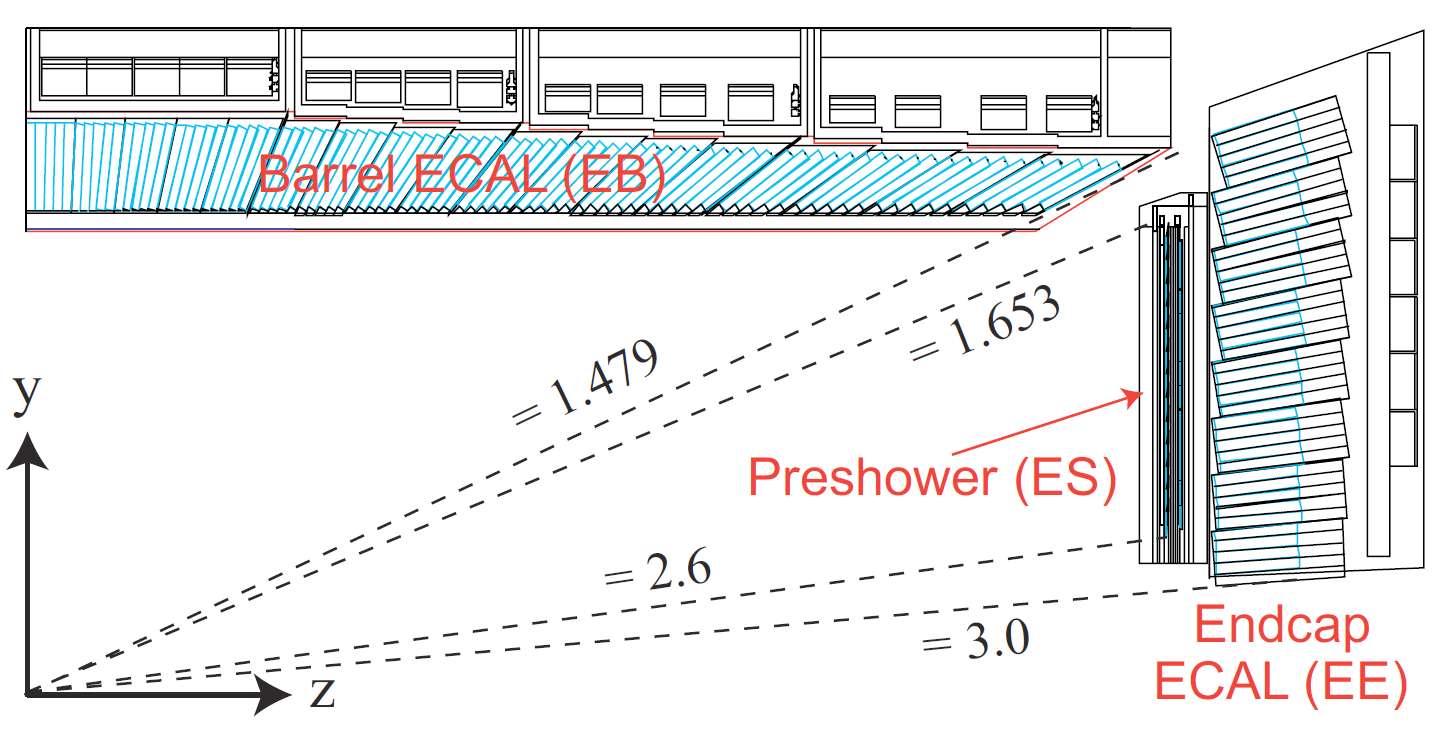
\includegraphics[width=6.5cm]{Chapter2/ECAL_positioning.png}
\caption{A layout of the CMS Electromagnetic calorimeter displaying the arrangement of crystals in barrel and endcaps with the preshower present in front.}
\label{fig:ECAL}
\end{center}
\end{figure}
\vspace{-0.3in}

The ECAL barrel (EB) is extended upto $|\eta|$ $<$ 1.479 and consists of 61,200 crystals providing 360-fold granularity in $\phi$ and (2$\times$85)-fold
granularity in $\eta$ direction. The crystals are of trapezoidal shape having a front cross section of 22$\times$22$\unit{mm}^{2}$,
a rear cross section of 26$\times$26$\unit{mm}^{2}$ and
a length of 230\unit{mm}, equivalent to 25.8$X_{0}$ implying that it is able to contain 99.999$\cdots\%$ of $e/\gamma$ energy. These crystals are assembled
into 36 supermodules, each weighing around 3 tonnes and containing 1700 crystals. Each supermodule covers 20$^{^{\circ}}$ in $\phi$ and half barrel in $\eta$.
The avalanche photodiodes (APDs) are used as photo-detectors to capture the scintillating light generated in the crystals upon interaction. These are made up of
semiconducting silicon and have an active area of 5$\times$5$\unit{mm}^{2}$. The relatively low light yield of PbWO$_{4}$ crystals is compensated by the
signal amplification by APDs through avalanche process. In addition, insensitivity of APDs towards high magnetic field and high radiation environment, makes them
convenient for EB. 

The flat circular ECAL endcaps (EE) cover the barrel at both the ends in the pseudorapidity range 1.479 $<$ $|\eta|$ $<$ 3.0, each consisting of 7,324 crystals arranged
in 5$\times$5 crystal units, known as supercrystals. The trapezoidal crystals have a front face of
28.62$\times$28.62$\unit{mm}^{2}$, a rear face of 30$\times$30$\unit{mm}^{2}$
and a length of 220\unit{mm} (24.7$X_{0}$). Endcaps use vacuum phototriodes (VPTs) as photo-detectors since these can work in high radiation environment compared to
APDs. Each VPT has a diameter of 25\unit{mm} and an active area of 280$\unit{mm}^{2}$. In front of each ECAL endcap is present a high granularity sampling calorimeter,
known as ECAL Preshower (ES), made up of alternating layers of lead (passive medium) and silicon strips (active medium). It covers a pseudorapidity range of
1.653 $<$ $|\eta|$ $<$ 2.6 and forms a disc of 2.5\unit{m} circumference. The disc is about 20\unit{cm} thick and has a 50\unit{cm} diameter hole in the middle
for the passage of beam pipe. The principle aim of ES is to identify and stop overlapping photons coming from the decay of $\pi^{0}$ so as to prevent
false signals. The high density of lead stimulate quick showering, thereby resulting into the shower containment in
a very small volume. Around 95$\%$ of incident photons start showering in the first lead plane. 

Many contributions deteriorate the actual energy resolution of any realistic calorimeter. The energy resolution of ECAL
(for energies below 500\unit{GeV}) can be written in general as:
\begin{equation}
  \frac{\sigma}{E} = \frac{S}{\sqrt{E}} \oplus \frac{N}{E} \oplus C
\end{equation}
where $\oplus$ corresponds to quadratic sum which implies that the contributions of different terms are independent from each other. The first term $S$
is known as stochastic or sampling term. It considers the statistical fluctuations due to the shower fluctuations, lateral shower leakage,
photo-detector inefficiencies, efficiency loss due to the shower containment in the passive medium of preshower etc. The second term $N$ corresponds to the
noise term arising due to instrumental effects, light-attenuation, pileup effects etc. The last term $C$ is a constant term and it includes effects from
imperfections in calorimeter construction, inter-calibration errors, longitudinal shower leakage, fluctuation in energy deposition in the dead areas of calorimeter etc.


The test beam studies~\cite{Chatrchyan:2013dga} were performed using a block of 3$\times$3 crystals and various terms involved in energy resolution were computed. These terms
for barrel region are: $S$ = 2.8$\%$, $N$ = 124\unit{MeV} and $C$ = 0.3$\%$ while for endcap region are: $S$ = 5$\%$, $N$ = 500\unit{MeV} and $C$ = 0.3$\%$.

\paragraph{Hadronic calorimeter}
\hspace{\parindent} The CMS HCAL has been designed to measure energy of particles (hadrons) interacting via strong force. Hadrons interact with the material
of the detector through strong nuclear interactions, resulting into the production of a large number of
secondary hadrons, thereby activating a hadronic shower. A majority of these shower particles, around 90$\%$, are pions. Among these, the neutral pions ($\pi^{0}$)
decay electromagnetically into two photons, thereby generating a component of EM shower within a hadronic shower. The fraction of energy of a hadron taken off
by the EM component is denoted as $f_{\textrm{EM}}$ and it varies from event-to-event. This fraction depends on the energy of initial hadron and
varies from 30$\%$ for a 10\unit{GeV} hadron to 50$\%$ for a 100\unit{GeV} hadron. Also, a significant fraction of
shower particles lose their energy as nuclear binding energy in nuclear reactions. This energy does not appear as a signal in the calorimeter and therefore, dissipate as
invisible energy. As a consequence, the calorimeter signal for a hadron is usually smaller than an electron having same energy,
a phenomenon known as non-compensation, also denoted as $e/h$ ratio. These two features of hadron showers result into a non-linearity in
the energy measurement of hadrons by HCAL.

The shower profiles of hadrons are characterized by nuclear interaction length, $\lambda_{\textrm{int}}$ (expressed in $\unit{g/{cm}^{2}}$)
which is the mean distance traversed by a hadron before undergoing a nuclear interaction. Usually, the interaction length of a hadron is much larger than
the radiation length of an electron of same energy, e.g. in copper, $X_{0}$ = 1.4\unit{cm} while $\lambda_{\textrm{int}}$ = 15\unit{cm}. 
This implies that a large amount of material is required to contain a hadron of a particular energy compared to an electron of same energy, not
possible to achieve with homogeneous calorimeter. Therefore, the hadron calorimeter always use sampling configuration. A properly designed sampling detector achieves
compensation of hadronic signals by the use of various techniques and sampling fractions~\cite{Wigmans:1991cc}.

The HCAL~\cite{hcalTDR} is a sampling calorimeter constructed of a dense absorber material made up of brass$/$steel plates interleaved with plastic scintillator tiles,
which are read out via embedded wavelength-shifting (WLS) fibres. This configuration is chosen for both barrel and endcap regions of HCAL
due to the non-magnetic behaviour, high absorption length and
good mechanical strength of brass while long term stability and radiation hardness of plastic scintillators. The detector is assembled in such a way that it
does not have any cracks or dead areas in $\phi$. The scintillator
tiles emit blue-violet light upon particle interaction, which is then converted into green light by WLS fibres. These optical signals are then converted into
electronic signals by the use of Hybrid Photodiodes (HPDs).
The HCAL constitutes of four sections: HCAL Barrel (HB)~\cite{Abdullin:2008zzb},
HCAL Endcaps (HE)~\cite{Baiatian:2008zz}, HCAL Forward (HF)~\cite{Bayatian:2006jz}, and HCAL Outer (HO)~\cite{Abdullin:2008zza}. The HCAL, in association
with ECAL, provides the energy$/$direction measurements of hadrons. A schematic view of a section
of HCAL is presented in \fig{\ref{fig:HCAL}}.

\begin{figure}[h]
\begin{center}
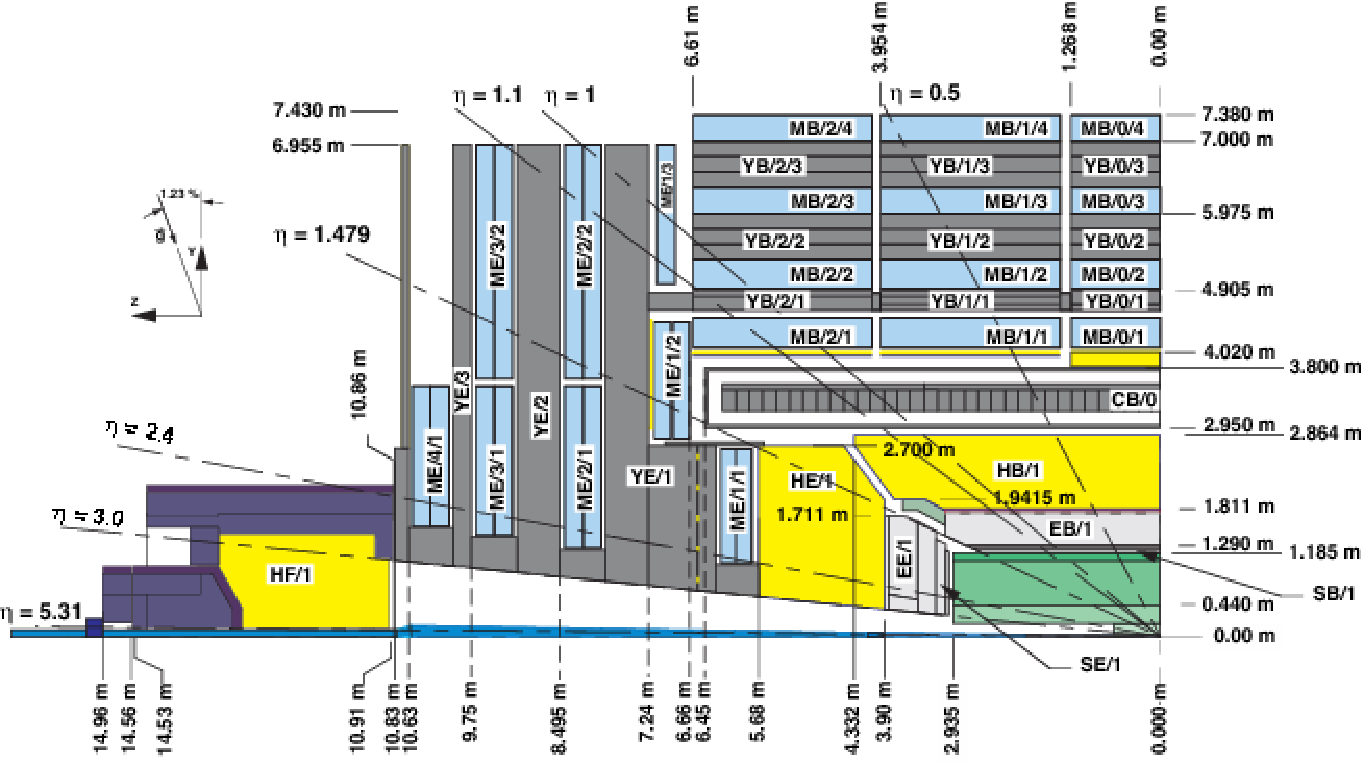
\includegraphics[width=13cm]{Chapter2/HCAL_layout.pdf}
\caption{A schematic view of a quadrant of the CMS Hadron calorimeter presenting different sub-detectors (in yellow color).}
\label{fig:HCAL}
\end{center}
\end{figure}
\vspace{-0.3in}

The HCAL barrel covers a pseudorapidity range of $|\eta|$ $<$ 1.3 and is made up of two half barrels, each made of 18 azimuthal wedges,
each covering 20$^{^{\circ}}$ in $\phi$. Each wedge is sliced into 16 absorber plates, with front and back plates made of
steel and rest made of brass (a Cu-Zn alloy). The plastic scintillating tiles with WLS fibres are arranged into trays containing many tiles and
are inserted between each plate to construct a sampling configuration. Each wedge is further partitioned into 4$\phi$ sectors while
the plastic scintillators are further partitioned into 16$\eta$ sectors, resulting into a segmentation of $\Delta\phi$ $\times$ $\Delta\eta$ = 0.087 $\times$ 0.087.
The HB is situated between EB (at $r$ = 1.77\unit{m}) and superconducting magnet (at $r$ = 2.95\unit{m}), resulting into highly constrained material amount.
The total thickness of HB corresponds to 5.82$\lambda_{\textrm{int}}$ at $\eta$ = 0 and 10.6$\lambda_{\textrm{int}}$ at $\eta$ = 1.3, ECAL also adds a thickness of
1.1$\lambda_{\textrm{int}}$ to HB material. In order to ensure the proper energy containment of hadronic showers, a complementary detector layer of same
configuration known as HO, is positioned outside the magnet coil which acts as a tail-catcher for any late starting showers.
It provides an additional thickness of 1-2$\lambda_{\textrm{int}}$ to HB showers. The high pseudorapidity region, 1.3 $<$ $|\eta|$ $<$ 3.0 has been
instrumented using HE on both sides of HB. The endcaps are made of 17 brass plate layers with plastic scintillator tiles accommodated in between. Including with EE,
it corresponds to a total thickness of around 10$\lambda_{\textrm{int}}$.

The high radiation environment (3.0 $<$ $|\eta|$ $<$ 5.0) near the beam pipe is armed with a more robust hadron forward (HF) calorimeter made up of quartz fibres
as active medium and steel as the absorber medium. The front face of HF is located at a distance of 11.2\unit{m} from the interaction point. The structure is
divided into 36 azimuthal wedges of steel, 18 wedges on each side of collision point and composed of 5\unit{mm} thick scintillator plates along with WLS fibres.     
A signal in the form of Cherenkov radiation is produced in HF when a charged particle from the shower enters the active medium (quartz)
with a velocity greater than that of light in the medium. The HF has been utilized
to improve the $\met$ measurements and identify$/$reconstruct very forward jets which can contain distinguishing features of many physics processes.
The HF is also used in the measurement of online luminosity of CMS.

The energy resolution of CMS HCAL is parametrized as: $\frac{\sigma}{E}$ = $\frac{A}{\sqrt{E}} \oplus B$,
%\begin{equation}
%  \frac{\sigma}{E} = \frac{A}{\sqrt{E}} \oplus B 
%\end{equation}
with the parameters, $A$ = 0.847\unit{GeV} and $B$ = 0.074 for HB and HE and $A$ = 1.98\unit{GeV} and $B$ = 0.09 for HF.

\subsubsection{Solenoidal magnet}
The CMS uses a large solenoid magnet~\cite{cmsMagnet} as its central device around which the detector has been constructed. In order to achieve precise
measurements and resolutions of energy$/$momenta of charged particles coming from the collisions, CMS has deployed a large magnetic field of 3.8\unit{T}.
A charged particle in a uniform magnetic field $\vec{B}$ experience a force equal to $F$ = $qvB\sin{\theta}$, where $q$ is the particle's charge, $\vec{v}$ is
the particle's velocity and $\theta$ is the angle between $\vec{v}$ and $\vec{B}$.
In this magnetic field, the particle will traverse a curve of radius $\frac{mv}{qB\sin{\theta}}$, $m$ being
the mass of particle, which implies that the particles of different initial velocities or momenta will be curved differently inside field $\vec{B}$. Therefore,
measurement of the angle and radius of curvature of charged particles inside $\vec{B}$ can be used to get an estimate of particle's momentum. Also, the momentum resolution
depends on the magnitude of magnetic field $\vec{B}$ and length of solenoid $L$ as $\frac{\Delta{p}}{p}$ = $\frac{p}{BL^{2}}$, stating that a large
resolution (less $\Delta{p}$) can be achieved by the use of a high magnetic field of large size.  

The CMS magnet as shown in \fig{\ref{fig:Magnet}} is a solenoidal magnet made of superconducting Nb-Ti coils which produce an intense magnetic field of 3.8\unit{T} when
a current of 19,500\unit{Ampere} is passed through them.
The magnet with a length of 13\unit{m} and an internal diameter of 5.9\unit{m} fit snugly the tracker and calorimeters inside.
It consists mainly of three parts: the coil, vacuum tank and yoke. The vacuum tank acts as a cryostat and provide the essential cooling to solenoid using liquid He.
The return yoke is made up of iron and is present outside the magnet coil reaching an outer diameter of 14\unit{m}.
It is responsible for return of magnetic flux with a field of 2\unit{T}.
The yoke is a 12-sided structure made up of 11 discs, 5 in barrel and 6 in endcaps, the muon chambers are interleaved in this.
The total energy stored inside the magnet amounts to around 2.6\unit{GJ}.

\begin{figure}[t]
\begin{center}
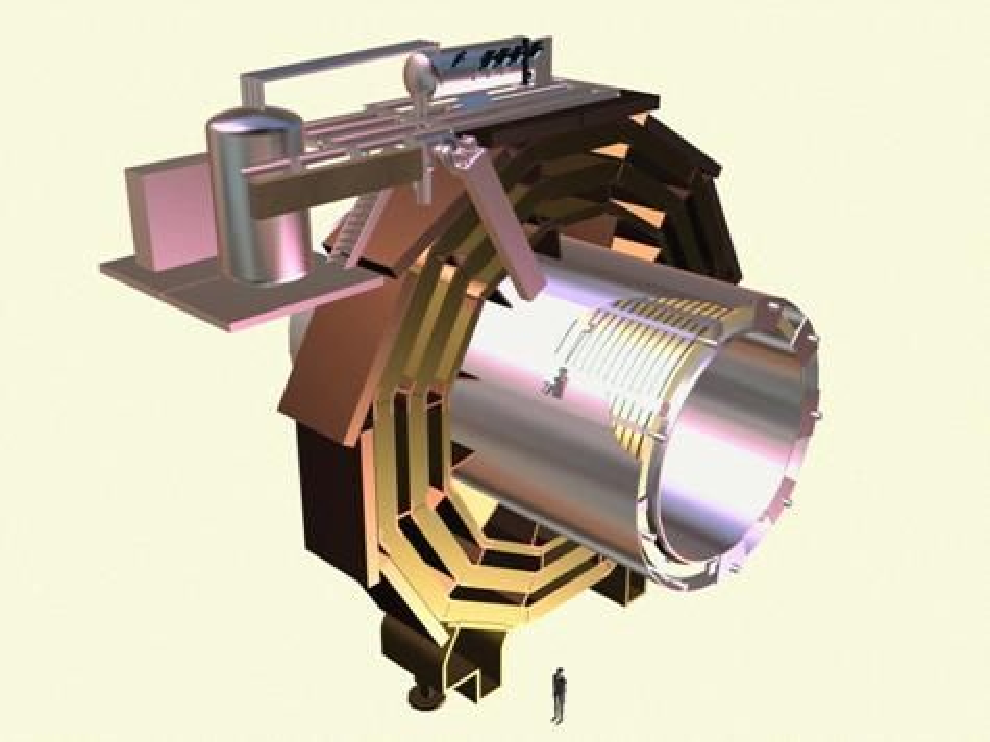
\includegraphics[width=9cm]{Chapter2/CMS_magnet.pdf}
\caption{A schematic view of the solenoidal magnet used in the CMS detector, showing the coil and the central return yoke.}
\label{fig:Magnet}
\end{center}
\end{figure}
%\vspace{-0.3in}

\subsubsection{Muon detector}
The CMS has been specifically designed for precise identification, momentum resolution and triggering of muons within a range $|\eta|$ $<$ 2.4 and $\pt$
$\leq$ 1\unit{TeV}. Muons, though interact electromagnetically,
do not lose much of their energy via bremsstrahlung owing to their high mass as compared to electrons. They interact primarily through ionization loosing
an energy on the average of 1-2$\unit{MeV/g/cm^{2}}$. Due to their less interacting nature, they penetrate the material of ECAL and HCAL, so the muon chambers for their
detection are installed at the very edge of the detector. 

The CMS muon~\cite{muonTDR} system has been divided into four stations interleaved with the return yoke and having a magnetic field of 2\unit{T}.
The barrel muon detector is also longitudinally divided into five wheels labelled as YB0, YB$\pm$1, YB$\pm$2, with each wheel being further divided in the azimuth
direction into 12 sectors of 30$^{^{\circ}}$ each. It uses
three different kind of detectors to observe muons: Drift Tubes (DTs), present in the barrel region upto $|\eta|$ $<$ 1.2; Cathode Strip Chambers (CSCs), present
in the endcap region for 0.9 $<$ $|\eta|$ $<$ 2.4; and Resistive Plate Chambers (RPCs), present in barrel as well as endcaps. Whenever a particle passes through these
chambers, it leaves its signature in the form of hits. Tracking the particle's position in multiple layers and combining the information from tracker, leads to
a precise determination of the position and momentum of the particle. The DTs$/$CSCs are good in position measurements while the RPCs provide
fast response, so a combination
of the three result into a robust muon detector. Diagrams representing the mechanical layout of CMS muon detector and the trajectory of muon through muon stations
is shown in \fig{\ref{fig:CMS_Muon}}.
 
\begin{figure}[h]
\begin{center}
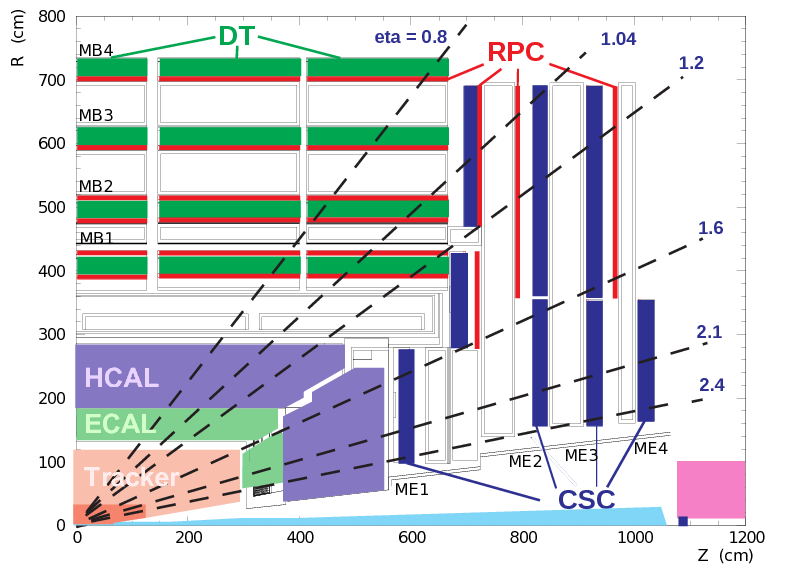
\includegraphics[width=8.5cm]{Chapter2/CMS_MuonDet.png}
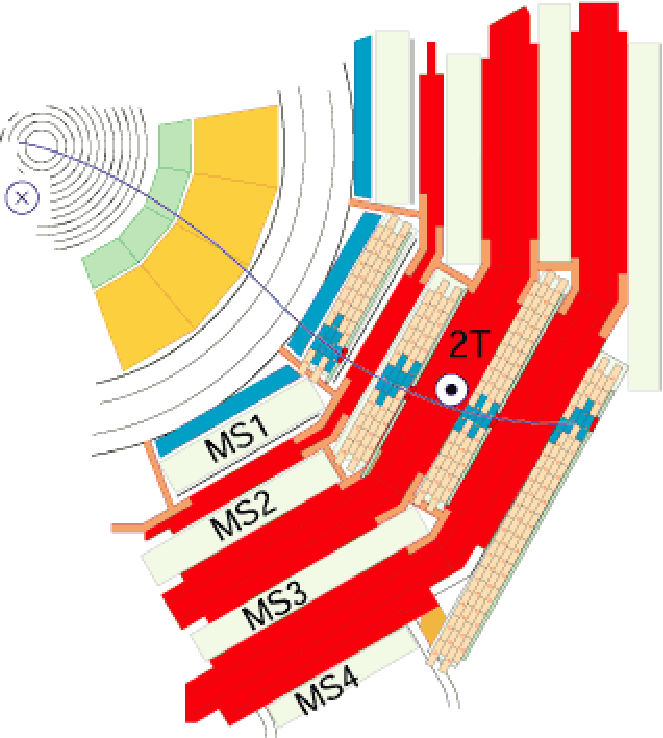
\includegraphics[width=5.5cm]{Chapter2/MuStations.pdf}
\caption{A schematic view of the solenoidal magnet used in CMS, showing the coil and the central return yoke. The trajectory of a muon through the muon stations is also presented.}
\label{fig:CMS_Muon}
\end{center}
\end{figure}
\vspace{-0.3in}

The drift tubes are organized into 4 stations labelled as MB1, MB2, MB3 and MB4, which forms concentric cylinders around the beam pipe.
Each of the inner three stations are composed of 12 drift chambers, with each chamber containing many drift tubes. These chambers are further grouped into
three superlayers denoted as SL1, SL2 and SL3, each consisting of four chambers. SL1 and SL3 provides
the co-ordinates of incident muons in $r-\phi$ plane while SL2 measures the co-ordinates in $r-z$ plane. The outermost station consists of two superlayers only. 
The choice of drift chambers is made in barrel due to the low particle rate and
uniform magnetic field. Each drift tube contains a anode wire of 50$\mu{m}$ diameter and two electrode plates to create electric field. The tube walls
are grounded and act as cathodes. The drift tube is filled with a gas containing a mixture of Ar (85$\%$) and CO$_{2}$ (15$\%$). The voltage difference between
wire and walls is about 1.8\unit{kV}. When a muon pass through the gas volume, it knocks off electrons which travel to the anode wire, carrying along
the information of incident particle. The DTs provide a signal gain of 10$^{5}$ and a drift time of 380\unit{ns}. 

The CSCs have been deployed in the high radiation and uneven magnetic field environment in the endcaps. Owing to their quick response time, high granularity and
radiation hardness, the CSCs are well qualified to identify muons in the range 0.9 $<$ $|\eta|$ $<$ 2.4, overlapping with DTs in 0.9 $<$ $|\eta|$ $<$ 1.2.
The CSC chambers are of trapezoidal shape placed perpendicular to the beam line and cover
10$^{^{\circ}}$-20$^{^{\circ}}$ in $\phi$. These are organized in 4 stations per endcap, labelled as ME$\pm$1, ME$\pm$2, ME$\pm$3 and ME$\pm$4, each station
containing a number of CSCs. Each CSC consists of an array of positive anode wires made of tungsten held perpendicular to the negative cathode strips made of
copper, in a gas mixture of Ar (40$\%$), CO$_{2}$ (50$\%$) and CF$_{4}$ (10$\%$). When a muon enters a CSC, it knocks off electrons from the gas atoms, which then
flock towards the anode wires resulting into an electron avalanche. The positive gas ions move towards cathode strips and induce a charge pulse. Since the
anode wires and cathode strips are present in perpendicular direction, these provide two position co-ordinates corresponding to each particle. This arrangement in
CSCs also results into fast response making them convenient for triggering. Each CSC is composed of six anode wires interleaved with seven cathode strips, providing
the measurements in $r-\phi$ plane. 

The RPCs are parallel plate gaseous detectors with fast response time and adequate position resolution making them suitable for
muon triggering. The RPCs are installed both in barrel (480 chambers)
and endcaps (432 chambers) with two chambers of rectangular shape per DT chamber in barrel and one chamber of trapezoidal shape per CSC chamber in endcaps.
The RPCs have the ability to tag a particle in a time frame much lesser than the bunch crossing time, making them ideal for triggering. The RPC is composed of
two gaps, each operating in avalanche mode and read-out strips are inserted in-between. The total signal induced by the RPC is sum of signal induced in each gap.
However, in order to ensure proper stability and operation of the RPC, an intensive control  of humidity, temperature and pressure is required.  

The muon system of CMS is made up of around 25000$\unit{m^{2}}$ area and more than a million readout channels.
Considering only the muon system without any information from
tracker (stand-alone muon), a momentum resolution of around 9$\%$ is obtained for a muon of $\pt$ $\leq$ 200\unit{GeV}
in low $\eta$ region. For a high $\pt$ muon ($\sim$ 1\unit{TeV}), the resolution varies from 15-40$\%$ for different $\eta$.
Adding tracker information (global muon) results into an improvement in momentum resolution of around 1$\%$ for low $\pt$ muons and around
5$\%$ for high $\pt$ muons. 


\subsubsection{CMS upgrade during Long Shutdown 1}
During LS1 in 2013-2015, minor repair and maintenance work were performed on most of the CMS sub-systems, except for
some major improvements that include: Installation of new pixel tracker layer (explained in \sectn{\ref{Se:CMS_tracker}}) which was actually
done after LS1 and during the technical stop at the
end of 2016, installation of new photo-detectors to improve signal-to-noise ratio in HCAL outer barrel, installation of the fourth RPC disk in the endcap region of
the muon detector which was actually the part of the first CMS technical design report and installation of around 72 new chambers in CSC along with 468 old chambers.
The electronics have also been updated to handle high collision rates.

\subsection{CMS Trigger and Data Acquisition System} \label{Se:CMS_trigger}
Most of the LHC collision data consists of ``soft'' particles which do not participate in any interesting process.
Also, at each bunch crossing, the collisions amount to a raw data of approximately 1\unit{MB}, which at the crossing rate of 40\unit{MHz} (25\unit{ns}), results into
around 40\unit{TB} data per second. It is almost impossible to store and process such a large amount of data.
Therefore, to reduce the data rate while keeping the potentially
interesting events for further analysis, a hardware and software based automated system, referred to as the CMS
trigger system\cite{triggerTDR} has been designed together with a
Data AcQuisition (DAQ) system~\cite{daqhltTDR}, as shown in figure \fig{\ref{fig:CMS_DAQ}}.
The trigger system consists of two layers: a hardware based trigger known as Level-1 (L1) trigger and a software
based trigger known as the High Level Trigger (HLT), reducing the event rate to an average of a few 100\unit{Hz} to
a maximum of 1\unit{kHz}. The data passing through both the trigger levels is stored for offline physics analysis.
In order to obtain the required data rate, sometimes the
triggers are prescaled at L1 or at HLT level, thereby storing only a fraction of selected events.
DAQ acts as a bridge between the two trigger layers, it gathers data from first trigger layer, digitizes and build it and
pass it to second trigger layer.

\begin{figure}[h]
\begin{center}
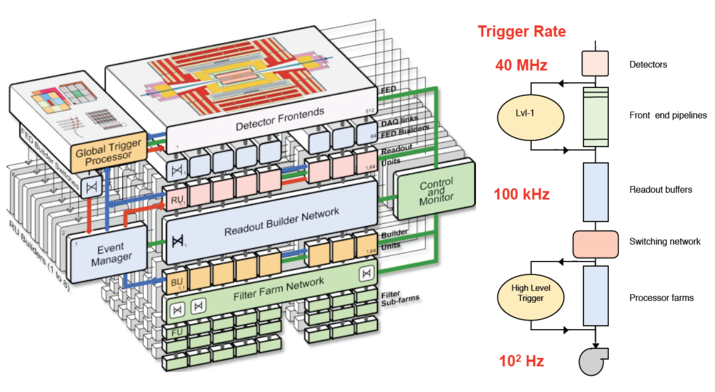
\includegraphics[width=13cm]{Chapter2/DAQsystem.png}
\caption{CMS Data Acquisition and trigger system.}
\label{fig:CMS_DAQ}
\end{center}
\end{figure}
\vspace{-0.3in}

\subsubsection{Level-1 trigger}
The Level-1 trigger of CMS is a set of hardware based triggers that rely on custom electronics. It has been designed to produce an output data
rate limit of 100\unit{kHz}. The L1 triggers are implemented as custom hardware processors and considers only low resolution, coarsely segmented data
from ECAL, HCAL and muon systems while keeping the high resolution data in the pipelined memories present in the front-end electronics. 
The L1 stores data in pipeline for 3.2${\mu{s}}$ during which it transmit its decision to detector electronics. 
The L1 trigger consists of a number of hardware components including field-programmable gate-array (FPGA) technology, ASICs and programmable lookup tables (LUTs).
A block diagram representing the architecture of L1 trigger system is shown in \fig{\ref{fig:CMS_L1}}.

\begin{figure}[h]
\begin{center}
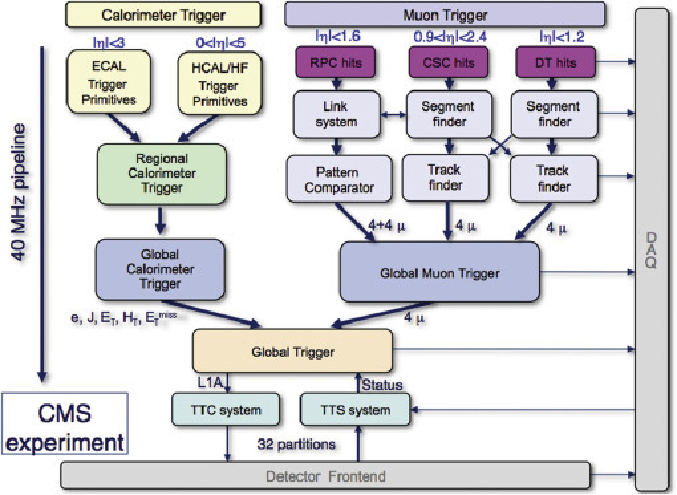
\includegraphics[width=10cm]{Chapter2/CMS_L1_trigger.pdf}
\caption{An architecture of CMS Level-1 trigger system.}
\label{fig:CMS_L1}
\end{center}
\end{figure}
%\vspace{-0.3in}
The L1 trigger consists of local, regional and global components. At the top are the local triggers, also known as Trigger Primitive Generators (TPGs),
which takes the information from the energy deposits in calorimeter towers and hit patterns in muon chambers. The information from TPGs are then passed on
to the regional triggers. The regional calorimeter triggers (RCTs) makes use of this information and forms sorted and ranked trigger
objects like electrons, photons and jets. The regional muon triggers (RMTs) join the segments and complete the tracks along with assigning physical parameters to them.
The regional triggers passes these objects along with various information to the Global Calorimeter Triggers (GCTs) and Global Muon Triggers (GMTs)
which sort out the highest ranked calorimeter and muon candidates along with determining various physics parameters like $\et$, $\met$, number of jets, $\HT$ etc.
This information from GCTs and GMTs are then passed on to the Global triggers (GTs),
the top level entity of L1 hierarchy, which makes the final decision of keeping or rejecting the event
by applying the programmable topological cuts and energy thresholds on the objects and issues the final Level-1 Accept (L1A) decision. The L1A is then
passed on to the Trigger Timing and Control (TTC) system for transferring it further to the detector front-end, from where it goes into the DAQ system.
The TTC also interfaces with the LHC machine to
provide clock and orbit information. The GT sends a command by the use of TTC in order to keep all the detectors and their electronics well in synchronization.

\subsubsection{High level trigger}
The CMS high level trigger accepts the output of L1 trigger and process it further by using a software (written mostly in C$++$)
based trigger system implemented in a filter farm consisting of more than thousand commercial processors. All major aspects of offline reconstruction code
are included in the filter farm software and is designed to reduce data rate to a minimum of few 100\unit{Hz}.
The average time taken in HLT processing is around 100\unit{ms}.
It employs the use of high resolution data and utilize many sophisticated algorithms to identify interesting events for
further storage. The HLT is based on highly flexible programming environment such that
the changes in the algorithms can be easily done to improve the various selections and to deal with unexpected experimental conditions.  
A set of algorithms that reconstruct the physics candidates (known as producers) and apply various selections to the reconstructed objects
(known as filters) is known as a ``trigger path''; a number of trigger paths together constitute a ``HLT trigger menu''.
Within a trigger path, the various algorithms are arranged in an increasing order of complexity, with the most complex algorithms like the b-tagging, are executed 
in the end. Events that pass any of the trigger paths within a trigger menu are considered for further analysis and are sent to storage manager where
these are stored on disks and are sent to CMS Tier-0 system present at CERN for offline processing and permanent storage.

\subsubsection{Data acquisition system}
The CMS DAQ mainly work as a carrier that gathers the data stored in detector's front-end modules at the Level-1 accept rate
and deliver it to HLT filter farms for further processing. 
It operates at an input data rate of 100\unit{kHz}, the output rate of L1 trigger. The complete processing of DAQ is summarized as follows:
First of all, the front end systems (FESs) store data continuously in 40\unit{MHz} pipelined buffers. As the synchronous L1 trigger comes, data are extracted
from FES via TTC and pushed into front end drivers (FEDs). The FEDs digitize, convert and zero suppress the data and then transfer it to
front end read out links (FRLs) that merge data from different FEDs. These FRLs are known as event builders as these built a complete event by assembling
the event fragments from all FEDs belonging to same L1. The data from FRLs are then transmitted into filter units (FUs). The HLT is mounted over FUs and use
its computing power to perform its operations. These FESs, FEDs, FRLs, FUs all forms the different parts of DAQ system. A Trigger-Throttling System (TTS)
has also been designed to protect DAQ against any back-pressures. 
\subsection{CMS data management}
The raw data after passing the various triggering stages, is managed further by the use of the LHC computing grid~\cite{Eck:840543}.
The grid is constituted of four levels$/$tiers, referred to as Tier-0 (T0), Tier-1 (T1), Tier-2 (T2) and Tier-3 (T3).
Each tier consists of a number of computer facilities and provides a set of dedicated services. 
The Tier-0 is the data center present at CERN, it contributes less than 20$\%$ of total grid computing capacity but it is responsible for maintaining a full copy
of raw data, for performing calibration and prompt reconstruction (prompt-reco) and for distributing the raw and prompt-reco data to Tier-1 centers. 
Tier-1 is a group of around 13 computer centers located in various part of the world and
joined together via optical-fibre links operating at a speed of 10$\unit{gigabytes/sec}$.
The T1 centers together maintain a second copy of raw
data, produce various Monte Carlo (MC) samples\footnote{simulated data samples, more information provided in \chap{\ref{ch:chapter3}}}
and re-reconstruct the raw data along with distributing it to various Tier-2 centers.
The T2 centers are the sites where physicists can log-in and perform their analysis within the CMSSW environment. These centers also produce the MC samples
and share them with T1 centers for storage and distribution to other sites. There are around 155 T2 sites distributed all over the world. 
The Tier-3 consists of local computing resources at various universities and institutes which individual users can access from any place around the world using grid,
and can use for storage and data analysis. 

The data present at various tiers are managed by the use of three data management tools~\cite{Giffels:2014tfa}:
Physics Experiment Data Export (PhEDEx)~\cite{Egeland:2008zz, Egeland:1196164}, Data Bookeeping Service (DBS)~\cite{Afaq:2007zz}
and Data Aggregation Service (DAS)~\cite{KUZNETSOV20101535}. The PhEDEx service provides data information access through the central PhEDEx database,
perform operations such as requesting data transfer or data deletion and transport the data among the different CMS sites along with keeping a track.
The DBS service keeps a metadata catalog of all the CMS data used by physicists as well as
the various production and analysis systems. The DAS service provides the user an overview of all the available datasets and keep a mapping between the datasets
and corresponding file blocks.
\subsection{CMS software and computing}
The CMS physics analyst perform various analyses using a collection of softwares based on C$++$ and python, referred to as the ``CMS Software frameWork''
(CMSSW)~\cite{cmsTDR}, installed at various T2 and T3 centers.
A number of services including simulations, calibration corrections or reconstruction etc. are supported by this framework.  
It consists of one main executable, known as cmsRun, along with many other plug-in modules, containing all the required codes for event processing.  
The cmsRun operates over a python configuration file that contains all the important information regarding the data and modules. 
The CMSSW software has been built over the concept of an ``Event''. An Event contains the information of a particular collision in different data
formats, a physics dataset consists of many events and are stored in the form of ROOT\footnote{ROOT is a data analysis framework}~\cite{Brun:1997pa} files.
A RAW data format contains the output of online trigger decisions and has a size of 1.5$\unit{MB}/$event, the size of RAW data in a simulated sample
is around 2$\unit{MB}/$event due to additional information. A RECO data
format contains the offline reconstructed data that includes the high level physics objects such as electrons, photons, jets, b-jets, muons, taus $\met$ etc., in
convenient format and has a size of 250$\unit{kB}/$event. Usually, a RECO data format contains a large amount of unwanted information,
so more compact data formats are obtained by filtering the RECO data. These data formats
includes Analysis Object Data (AOD) and mini Analysis Object Data (mini-AOD), used in almost all physics analyses. 

%It along with ATLAS chase the same physics goals but with the use of different technology as can be seen in \tab{\ref{Table:CMS_ATLAS_Comp}}. 
%\begin{table}[h!]
\begin{center}
\resizebox{16cm}{!}{
%\begin{tabular}{c !{\vrule width -1pt}c !{\vrule width -1pt}c !{\vrule width -1pt}c !{\vrule width -1pt}c !{\vrule width -1pt}c !{\vrule width -1pt}c !{\vrule width -1pt}c}  %%% !{\vrule width -1pt} to make column line width less, so that white space not visible in colored table. but not working very nicely.
\renewcommand{\arraystretch}{1.2}
\begin{tabular}{lcc}
\toprule
\belowrulesepcolor{Mygray}
\belowrulesepcolor{Mygray}
\belowrulesepcolor{Mygray}
\rowcolor{Mygray}[\dimexpr\tabcolsep+0.09pt\relax]  
System  & CMS & ATLAS \\
\aboverulesepcolor{Mygray}
\aboverulesepcolor{Mygray}
\aboverulesepcolor{Mygray}
\midrule
\bf{Tracker} & Silicon (pixel + microstrip) & Silicon (pixel + microstrip) \\
&                              & Gas (transition radiation) \\
\midrule
\bf{Electromagnetic} &  PbWO$_{4}$ crystals & Sampling (lead/liquid argon) \\
\bf{calorimeter} & &  \\
\midrule
\bf{Hadron} & Sampling (brass/plastic scintillator) & Sampling (steel/plastic scintillator) \\
\bf{calorimeter} &                                       & (copper/liquid argon) \\
\midrule
\bf{Muon detector} & Gas & Gas \\
\midrule
\bf{Magnet}      & Solenoid (around tracker        & Solenoid (around tracker)  \\
                 & and calorimeters)  &  Toroid (around muon)\\
&      Iron return yoke                      &  \\
\midrule
\bf{Magnetic field} & Approximately 4\unit{T} in solenoid & Approximately 2\unit{T} in solenoid \\
               & and 2\unit{T} in return yoke        & and 0.5--1\unit{T} in toroid \\
\bottomrule
\end{tabular}
}
\caption{A comparison of the technologies used in CMS and ATLAS.}
\label{Table:CMS_ATLAS_Comp}
\end{center}
\end{table}
\vspace{-0.4in}



